\section*{Anhang}
\addcontentsline{toc}{section}{Anhang}
\subsection*{Technische Aspekte der Simulation}
\addcontentsline{toc}{subsection}{Technische Aspekte der Simulation}
\begin{itemize}
	\item Git
	\item Java 8
	\item Maven
	\item Spring
	\item[?] Komplexeres UML
	\item Gebrauchsanweisung
	\item Lizenzen
\end{itemize}
\subsection*{Streudiagramme der Ergebnisse}
\addcontentsline{toc}{subsection}{Streudiagramme der Ergebnisse}
Die Streudiagramme dieser Arbeit wurden mit der Website \href{http:plot.ly/plot}{Plotly} erzeugt.
\subsubsection*{Einzelner lernender Fahrer}
\begin{figure}[H]
	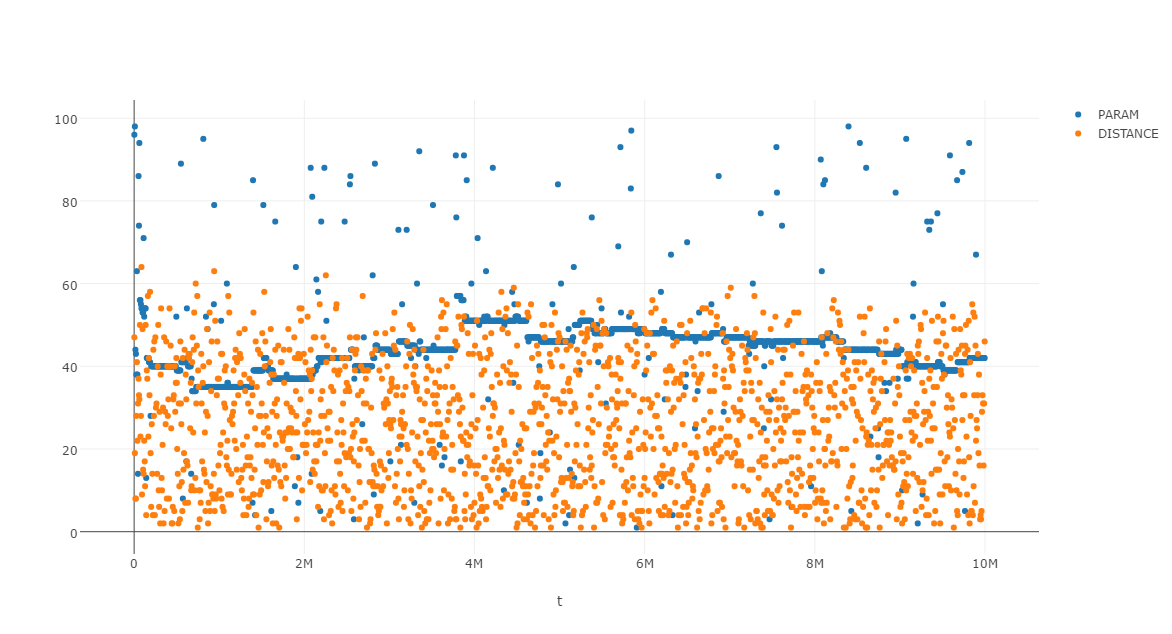
\includegraphics[width=0.8\textwidth]{analyse/SingleMutant/blockcount1.png}
	\caption{\emph{Block-Count}-Heuristik bei 1 Auto pro Minute und einem lernenden Fahrer}\label{fig:ap_sm_bc_1}
\end{figure}
\begin{figure}[H]
	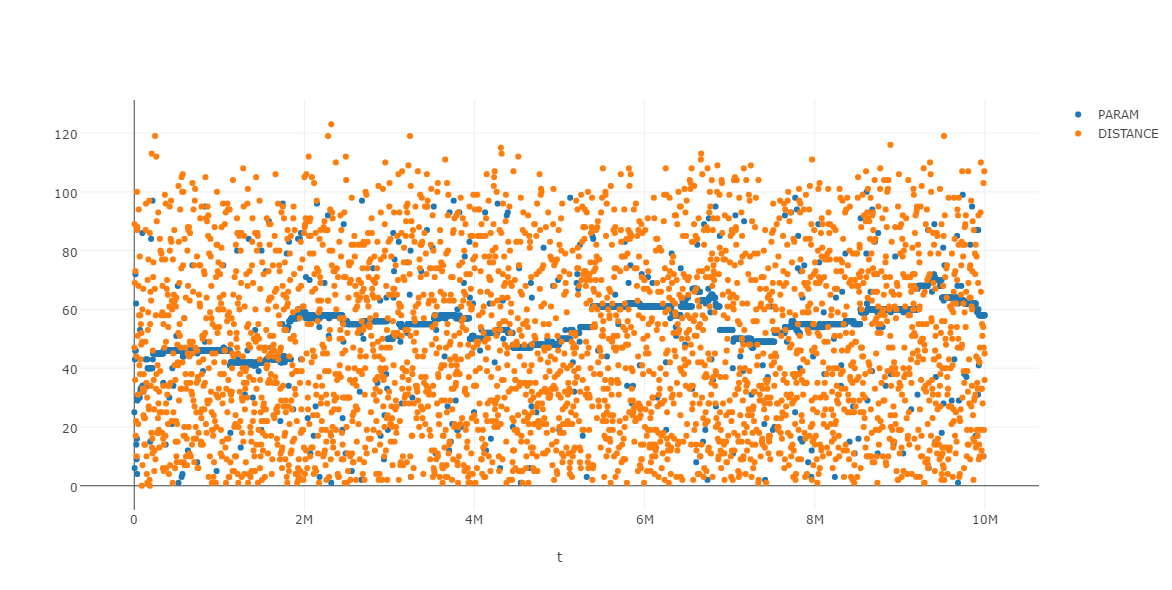
\includegraphics[width=0.8\textwidth]{analyse/SingleMutant/blockcount2.png}
	\caption{\emph{Block-Count}-Heuristik bei 2 Autos pro Minute und einem lernenden Fahrer}\label{fig:ap_sm_bc_2}
\end{figure}
\begin{figure}[H]
	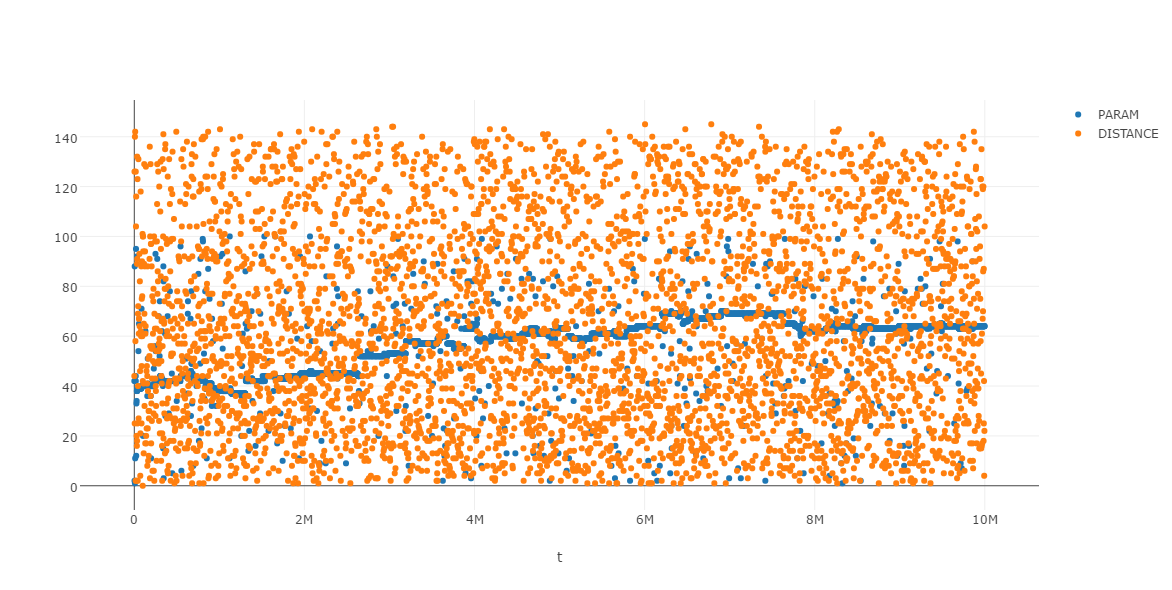
\includegraphics[width=0.8\textwidth]{analyse/SingleMutant/blockcount4.png}
	\caption{\emph{Block-Count}-Heuristik bei 4 Autos pro Minute und einem lernenden Fahrer}\label{fig:ap_sm_bc_4}
\end{figure}
\begin{figure}[H]
	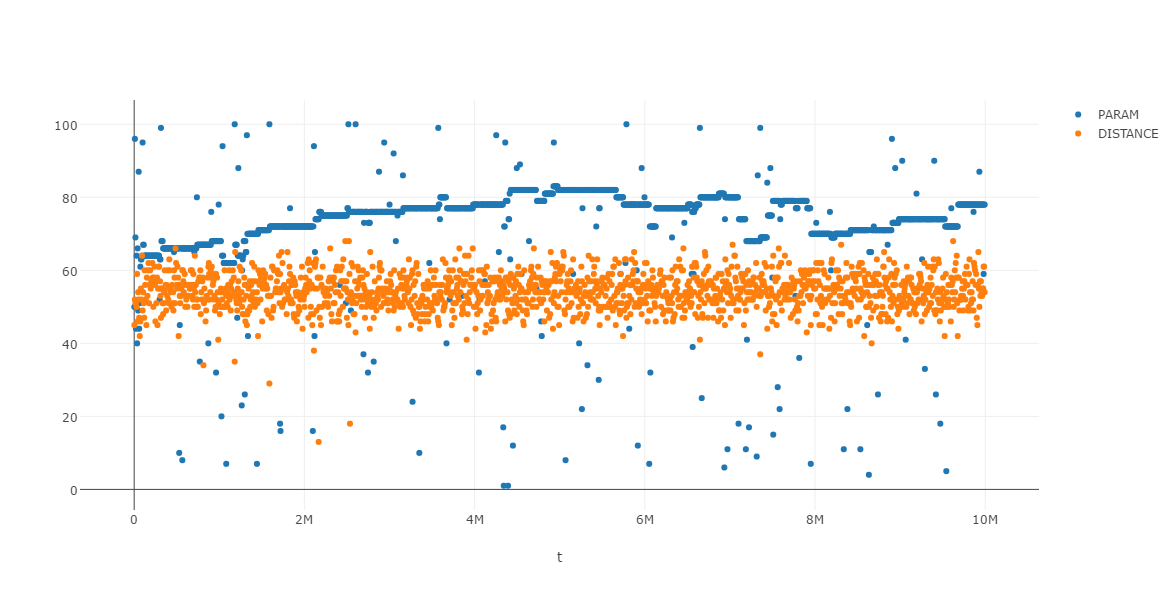
\includegraphics[width=0.8\textwidth]{analyse/SingleMutant/carcount1.png}
	\caption{\emph{Car-Count}-Heuristik bei 1 Auto pro Minute und einem lernenden Fahrer}\label{fig:ap_sm_cc_1}
\end{figure}
\begin{figure}[H]
	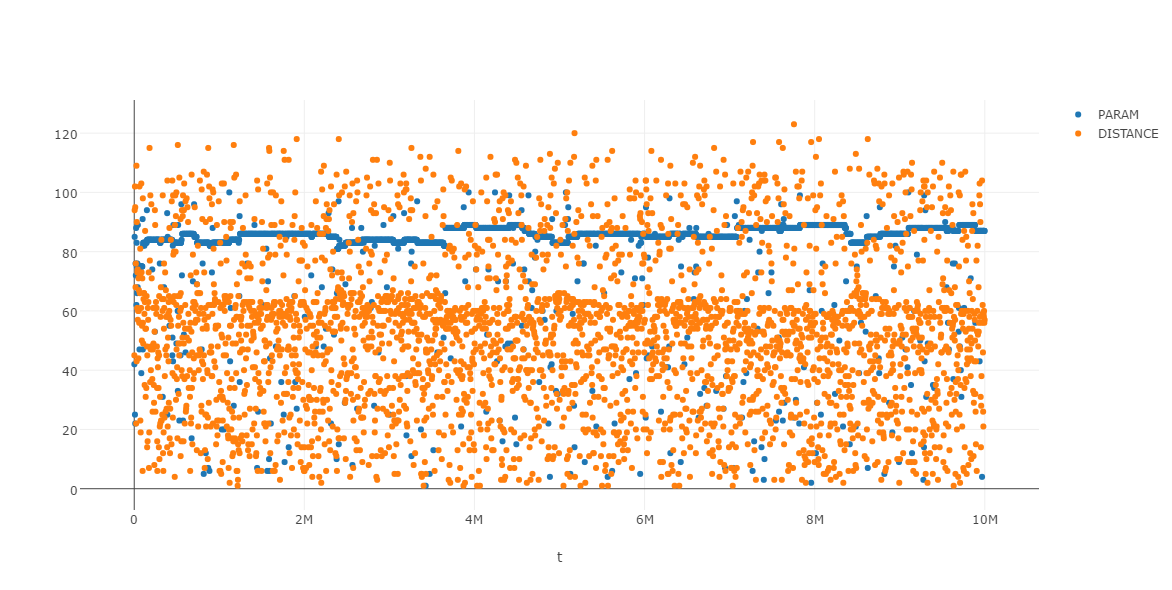
\includegraphics[width=0.8\textwidth]{analyse/SingleMutant/carcount2.png}
	\caption{\emph{Car-Count}-Heuristik bei 2 Autos pro Minute und einem lernenden Fahrer}\label{fig:ap_sm_cc_2}
\end{figure}
\begin{figure}[H]
	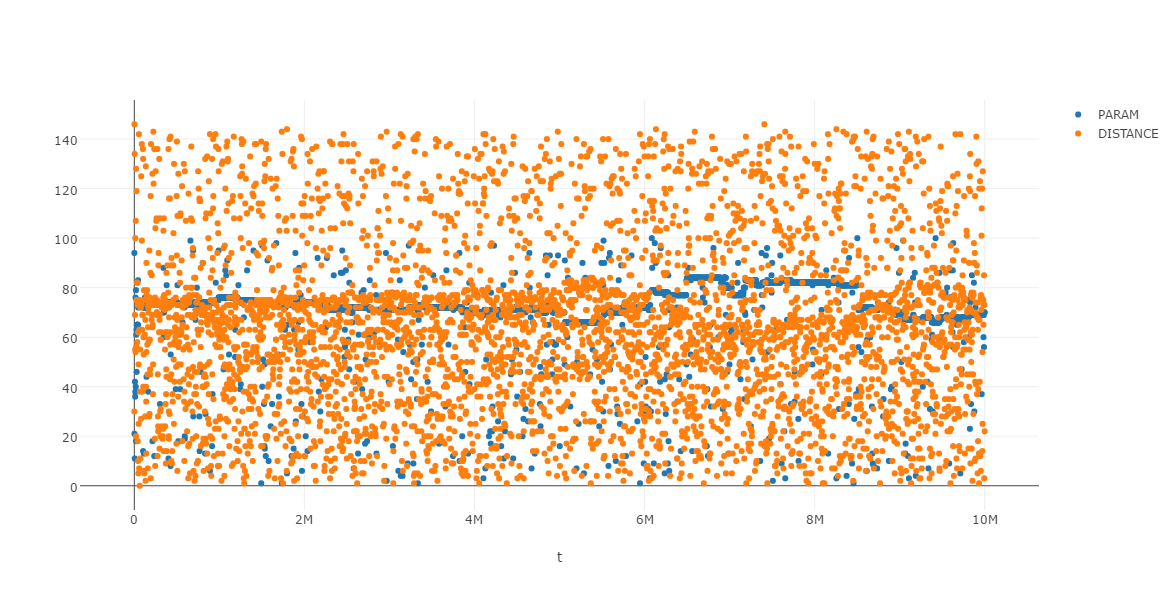
\includegraphics[width=0.8\textwidth]{analyse/SingleMutant/carcount4.png}
	\caption{\emph{Car-Count}-Heuristik bei 4 Autos pro Minute und einem lernenden Fahrer}\label{fig:ap_sm_cc_4}
\end{figure}
\begin{figure}[H]
	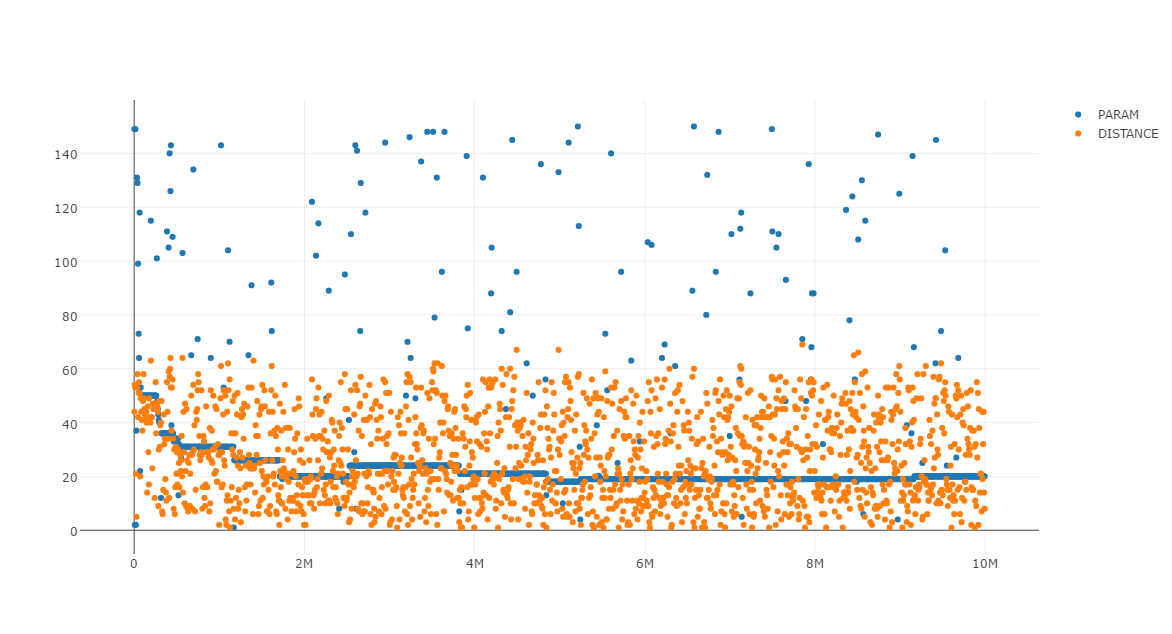
\includegraphics[width=0.8\textwidth]{analyse/SingleMutant/fixeddistance1.png}
	\caption{\emph{Fixed-Distance}-Heuristik bei 1 Auto pro Minute und einem lernenden Fahrer}\label{fig:ap_sm_fd_1}
\end{figure}
\begin{figure}[H]
	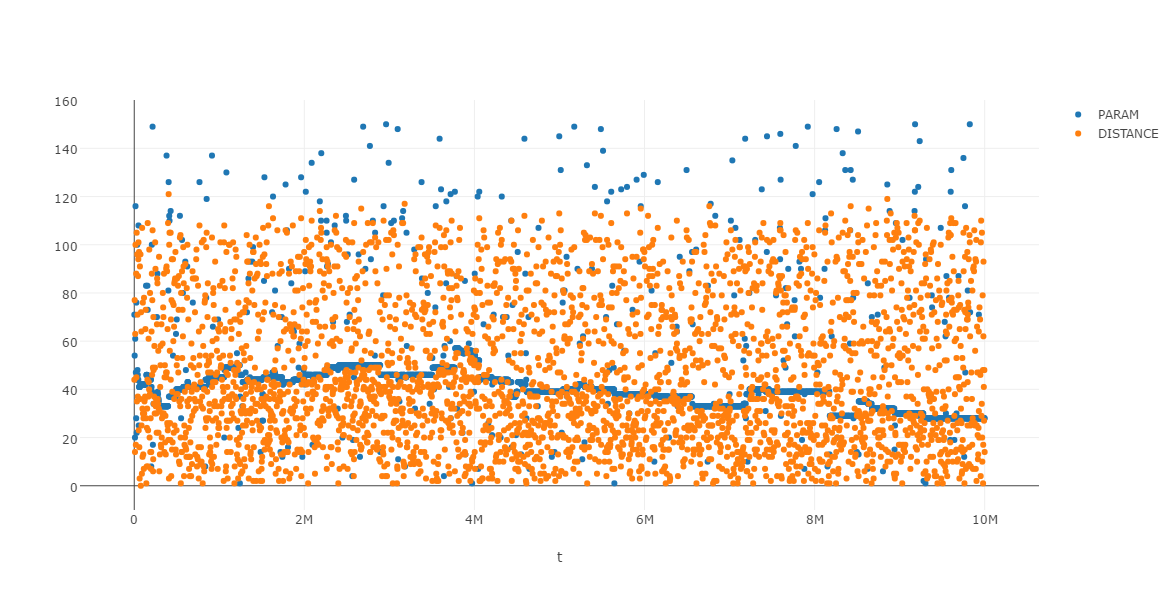
\includegraphics[width=0.8\textwidth]{analyse/SingleMutant/fixeddistance2.png}
	\caption{\emph{Fixed-Distance}-Heuristik bei 2 Autos pro Minute und einem lernenden Fahrer}\label{fig:ap_sm_fd_2}
\end{figure}
\begin{figure}[H]
	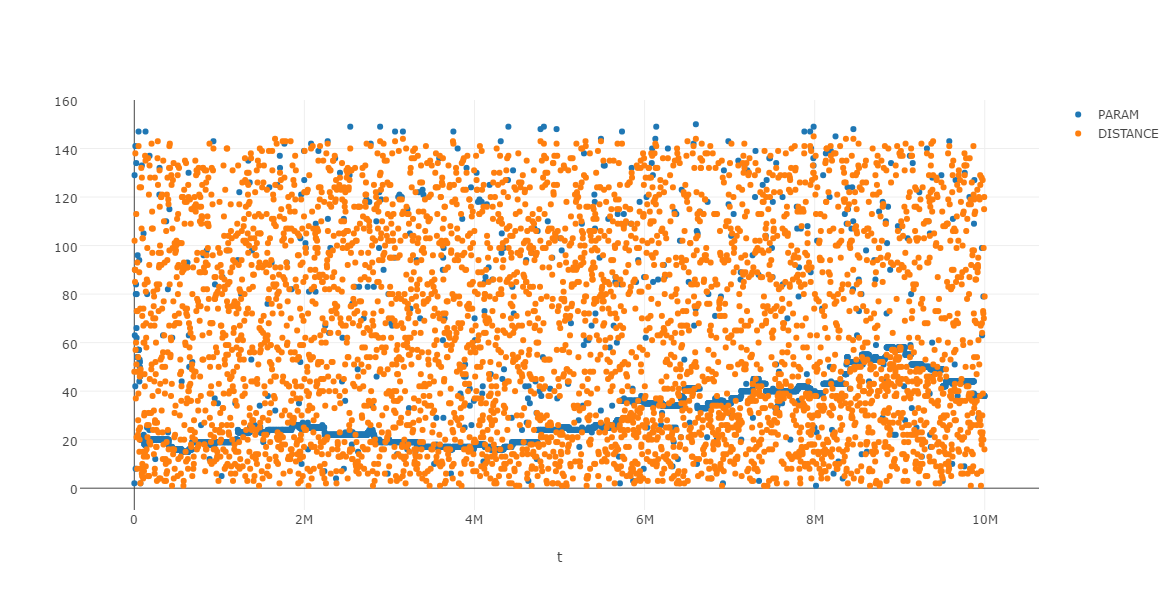
\includegraphics[width=0.8\textwidth]{analyse/SingleMutant/fixeddistance4.png}
	\caption{\emph{Fixed-Distance}-Heuristik bei 4 Autos pro Minute und einem lernenden Fahrer}\label{fig:ap_sm_fd_4}
\end{figure}
\begin{figure}[H]
	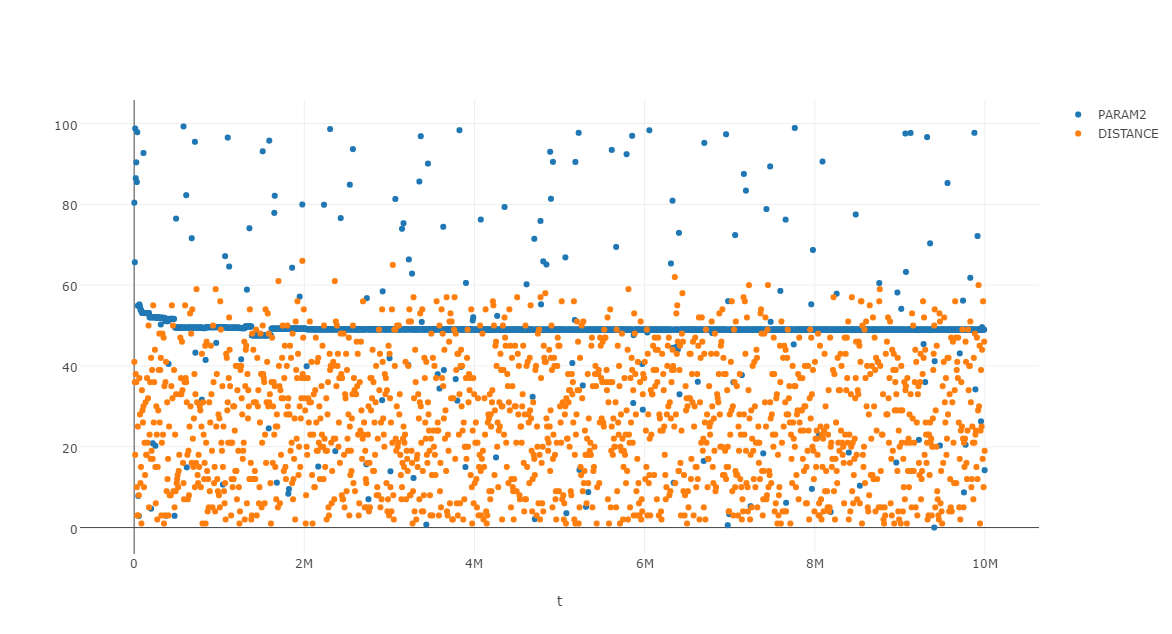
\includegraphics[width=0.8\textwidth]{analyse/SingleMutant/linopzt1.png}
	\caption{Schranke der \emph{Linear-Operator}-Heuristik bei 1 Auto pro Minute und einem lernenden Fahrer}\label{fig:ap_sm_loz_1}
\end{figure}
\begin{figure}[H]
	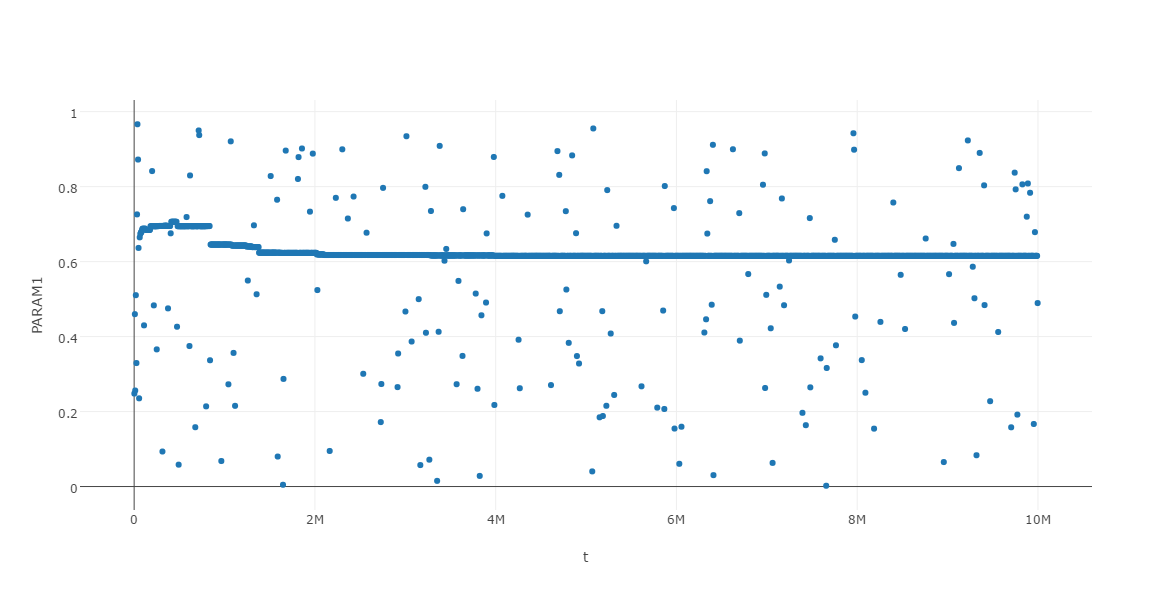
\includegraphics[width=0.8\textwidth]{analyse/SingleMutant/linopa1.png}
	\caption{Geschwindigkeit der \emph{Linear-Operator}-Heuristik bei 1 Auto pro Minute und einem lernenden Fahrer}\label{fig:ap_sm_loa_1}
\end{figure}
\begin{figure}[H]
	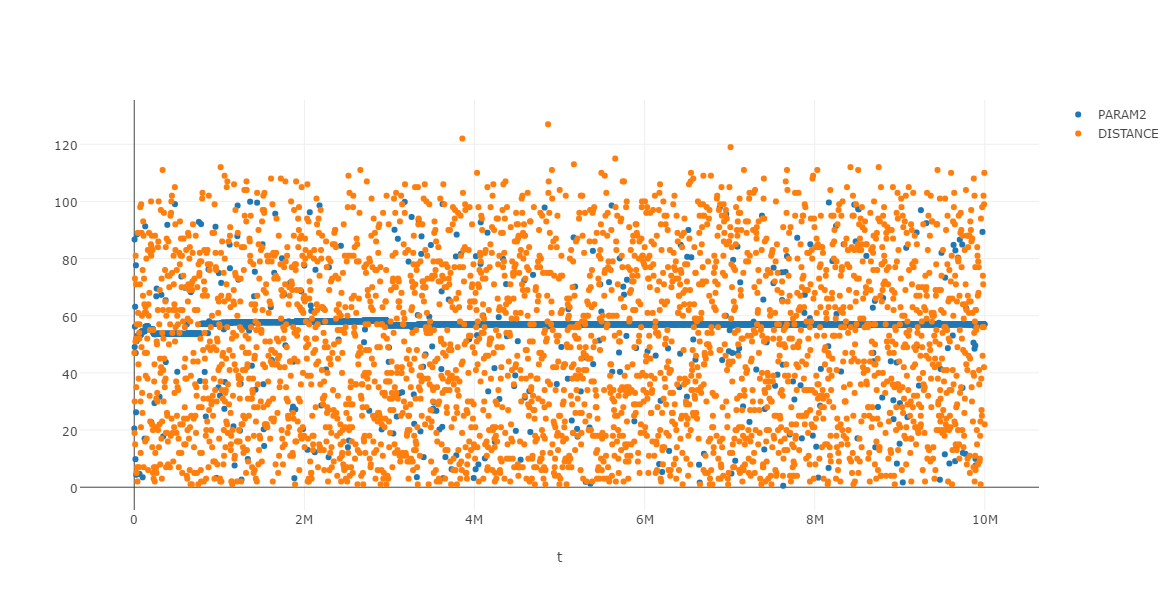
\includegraphics[width=0.8\textwidth]{analyse/SingleMutant/linopzt2.png}
	\caption{Schranke der \emph{Linear-Operator}-Heuristik bei 2 Autos pro Minute und einem lernenden Fahrer}\label{fig:ap_sm_loz_2}
\end{figure}
\begin{figure}[H]
	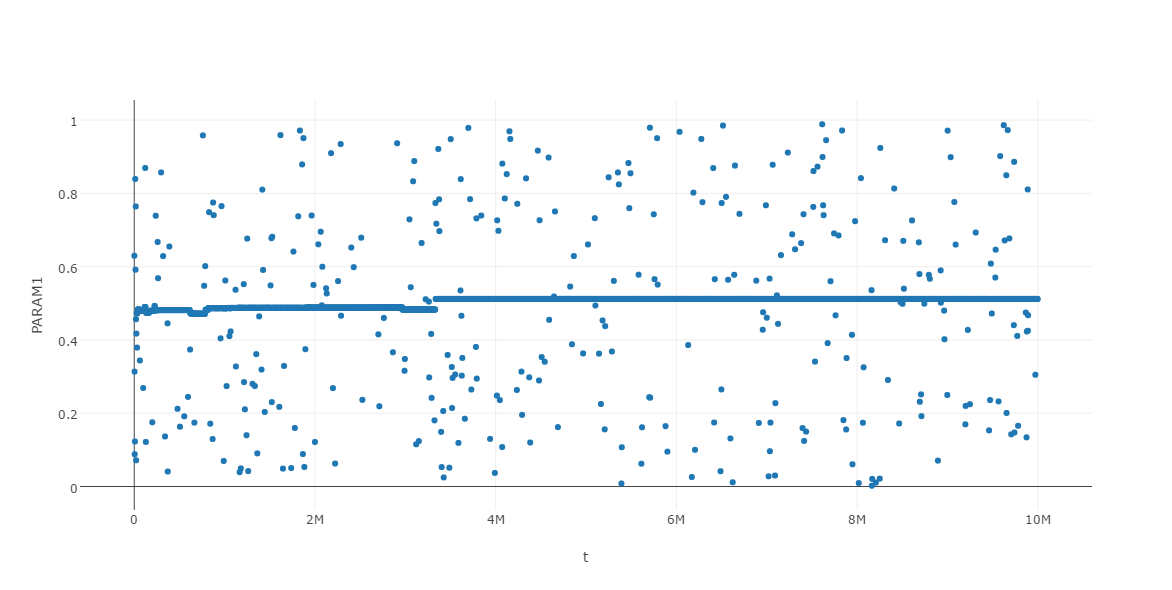
\includegraphics[width=0.8\textwidth]{analyse/SingleMutant/linopa2.png}
	\caption{Geschwindigkeit der \emph{Linear-Operator}-Heuristik bei 2 Autos pro Minute und einem lernenden Fahrer}\label{fig:ap_sm_loa_2}
\end{figure}
\begin{figure}[H]
	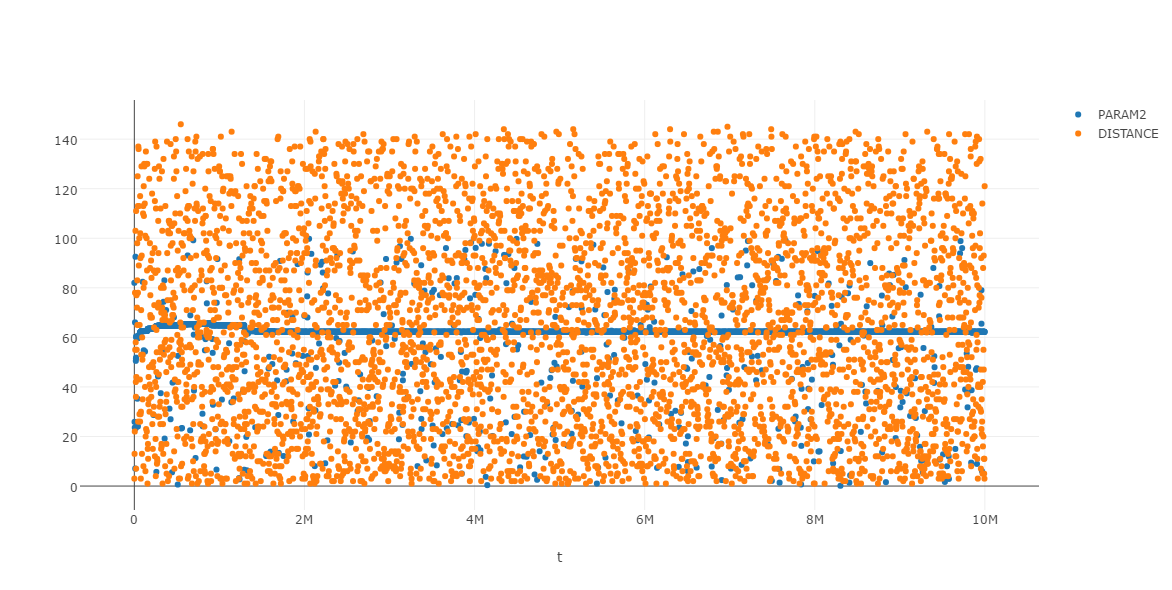
\includegraphics[width=0.8\textwidth]{analyse/SingleMutant/linopzt4.png}
	\caption{Schranke der \emph{Linear-Operator}-Heuristik bei 4 Autos pro Minute und einem lernenden Fahrer}\label{fig:ap_sm_loz_4}
\end{figure}
\begin{figure}[H]
	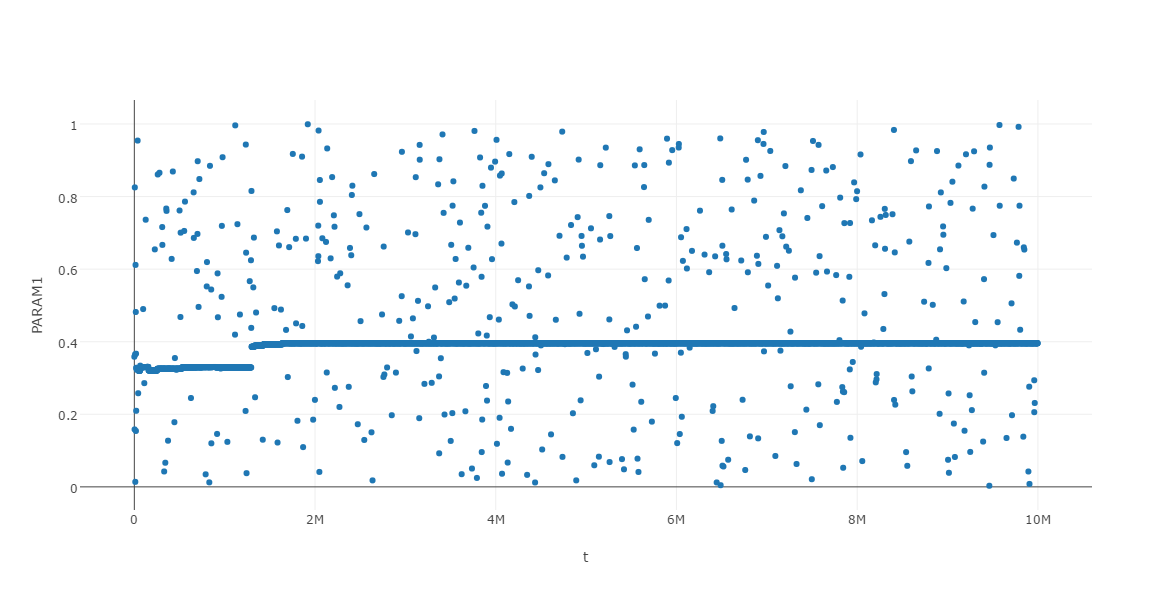
\includegraphics[width=0.8\textwidth]{analyse/SingleMutant/linopa4.png}
	\caption{Geschwindigkeit der \emph{Linear-Operator}-Heuristik bei 4 Autos pro Minute und einem lernenden Fahrer}\label{fig:ap_sm_loa_4}
\end{figure}
\begin{figure}[H]
	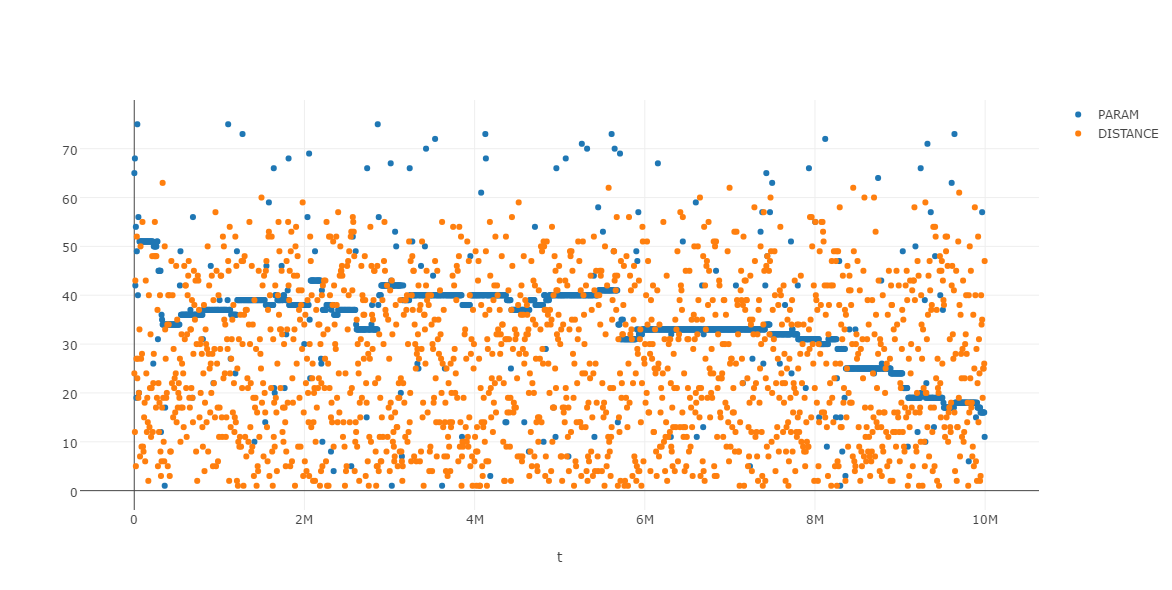
\includegraphics[width=0.8\textwidth]{analyse/SingleMutant/spacecount1.png}
	\caption{\emph{Space-Count}-Heuristik bei 1 Auto pro Minute und einem lernenden Fahrer}\label{fig:ap_sm_sc_1}
\end{figure}
\begin{figure}[H]
	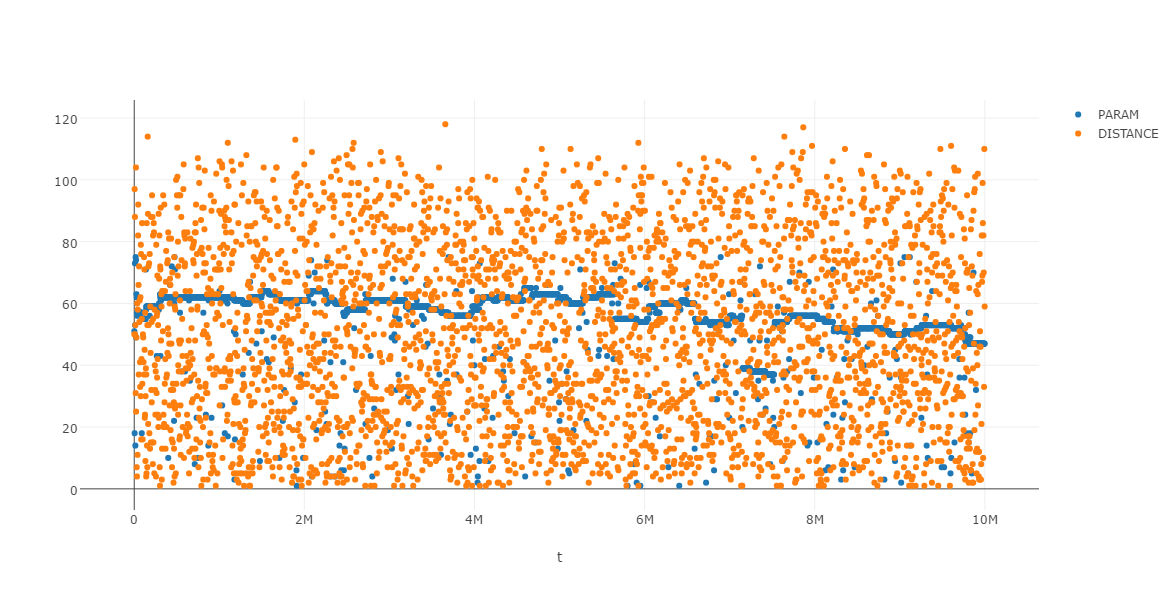
\includegraphics[width=0.8\textwidth]{analyse/SingleMutant/spacecount2.png}
	\caption{\emph{Space-Count}-Heuristik bei 2 Autos pro Minute und einem lernenden Fahrer}\label{fig:ap_sm_sc_2}
\end{figure}
\begin{figure}[H]
	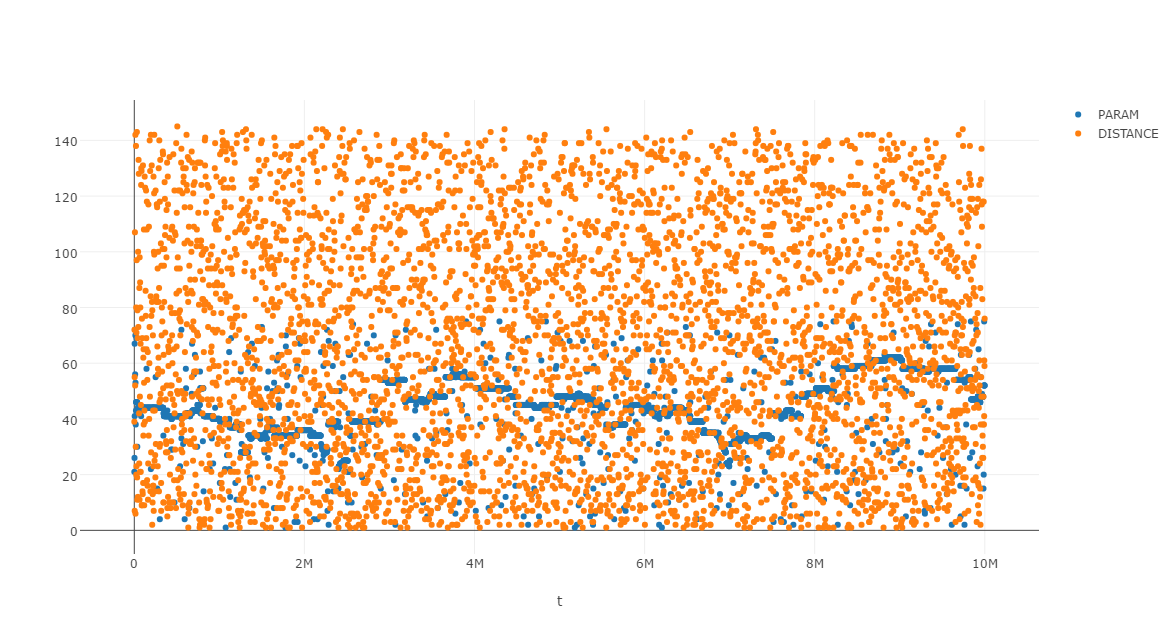
\includegraphics[width=0.8\textwidth]{analyse/SingleMutant/spacecount4.png}
	\caption{\emph{Space-Count}-Heuristik bei 4 Autos pro Minute und einem lernenden Fahrer}\label{fig:ap_sm_sc_4}
\end{figure}
\begin{figure}[H]
	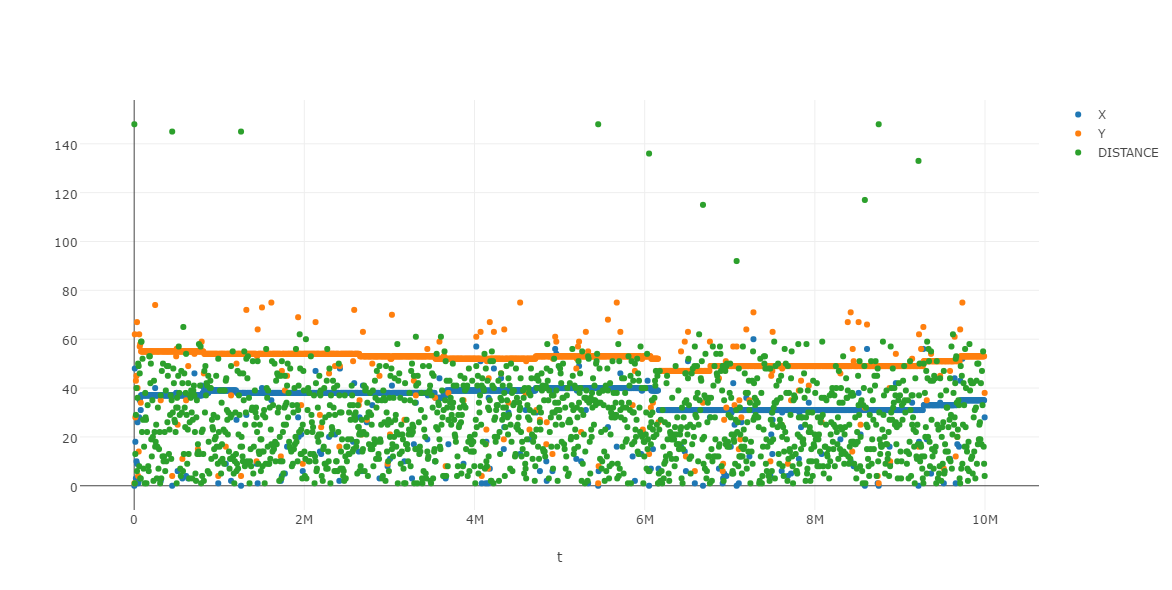
\includegraphics[width=0.8\textwidth]{analyse/SingleMutant/xy1.png}
	\caption{\emph{X-Out-Of-Y}-Heuristik bei 1 Auto pro Minute und einem lernenden Fahrer}\label{fig:ap_sm_xy_1}
\end{figure}
\begin{figure}[H]
	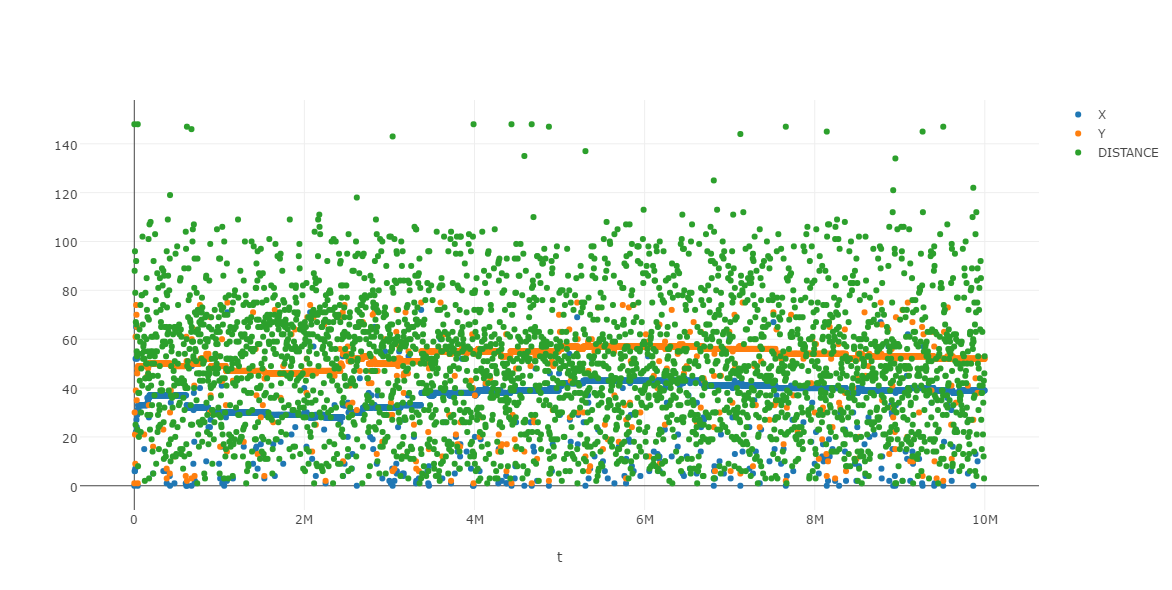
\includegraphics[width=0.8\textwidth]{analyse/SingleMutant/xy2.png}
	\caption{\emph{X-Out-Of-Y}-Heuristik bei 2 Autos pro Minute und einem lernenden Fahrer}\label{fig:ap_sm_xy_2}
\end{figure}
\begin{figure}[H]
	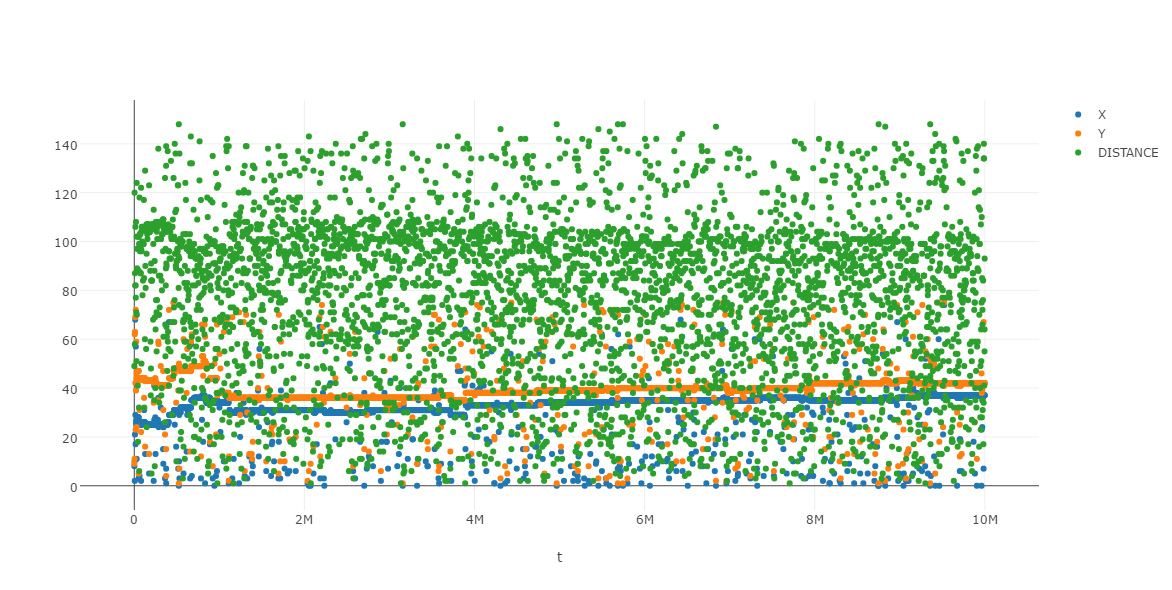
\includegraphics[width=0.8\textwidth]{analyse/SingleMutant/xy4.png}
	\caption{\emph{X-Out-Of-Y}-Heuristik bei 4 Autos pro Minute und einem lernenden Fahrer}\label{fig:ap_sm_xy_4}
\end{figure}

\subsubsection*{$20\%$ lernende Fahrer}
Im Gegensatz zum vorherigen Abschnitt sind die Heuristiken nun nach der durchgeführten Simulation sortiert.
\begin{figure}[H]
	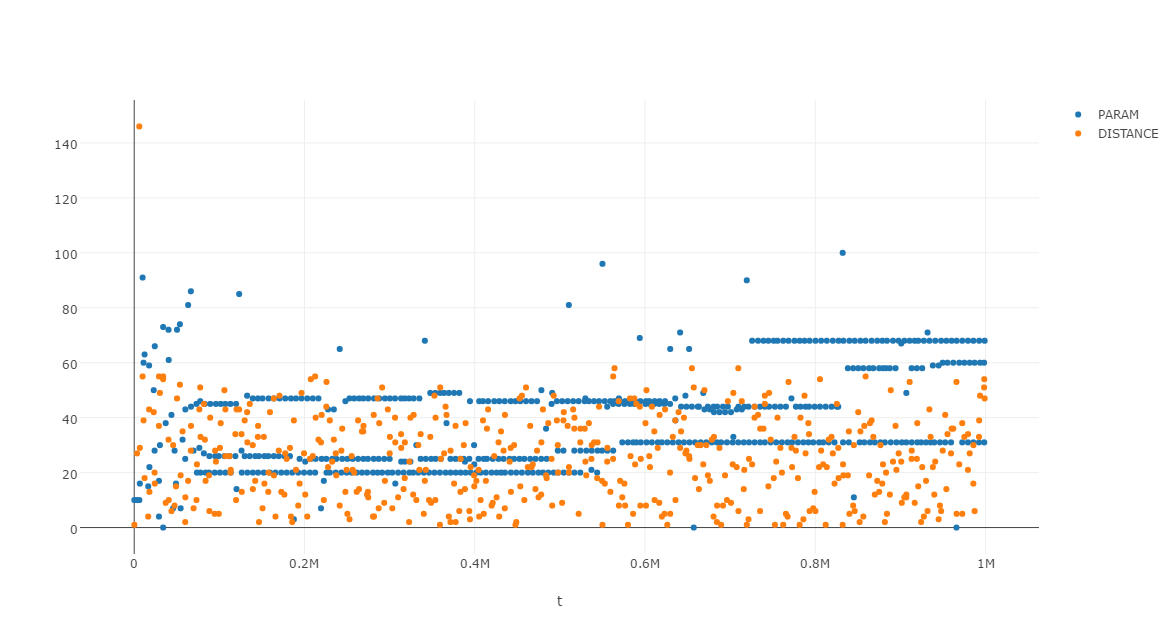
\includegraphics[width=0.8\textwidth]{analyse/SomeMutants/1pm/block1some.png}
	\caption{\emph{Block-Count}-Heuristik bei 1 Auto pro Minute und $20\%$ lernenden Fahrern}\label{fig:ap_pm_bs_1}
\end{figure}
\begin{figure}[H]
	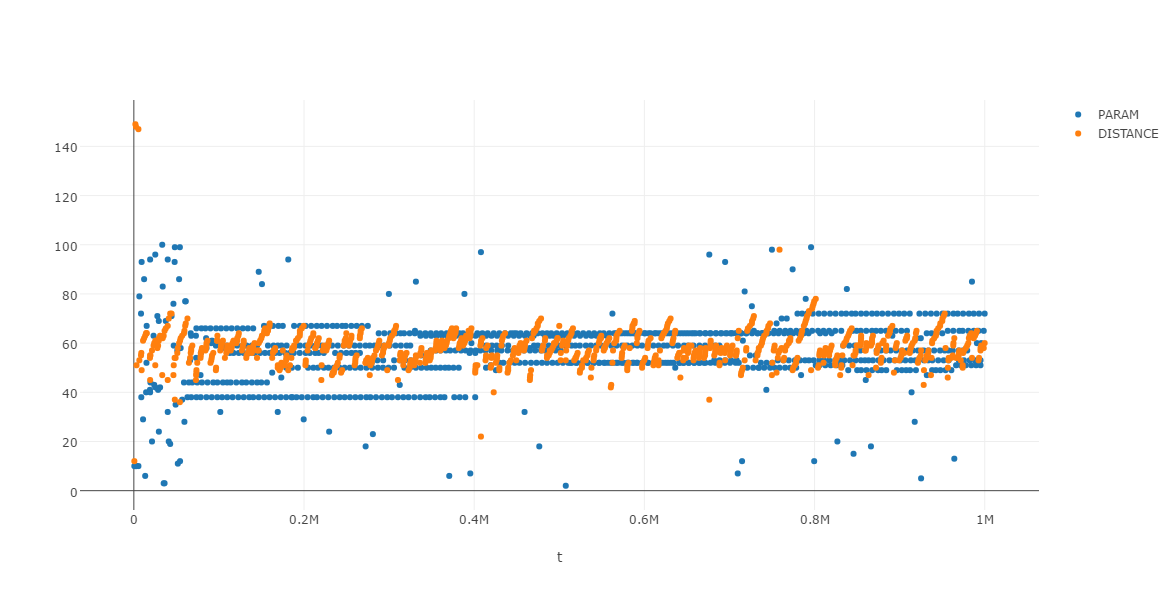
\includegraphics[width=0.8\textwidth]{analyse/SomeMutants/1pm/car1some.png}
	\caption{\emph{Car-Count}-Heuristik bei 1 Auto pro Minute und $20\%$ lernenden Fahrern}\label{fig:ap_pm_cc_1}
\end{figure}
\begin{figure}[H]
	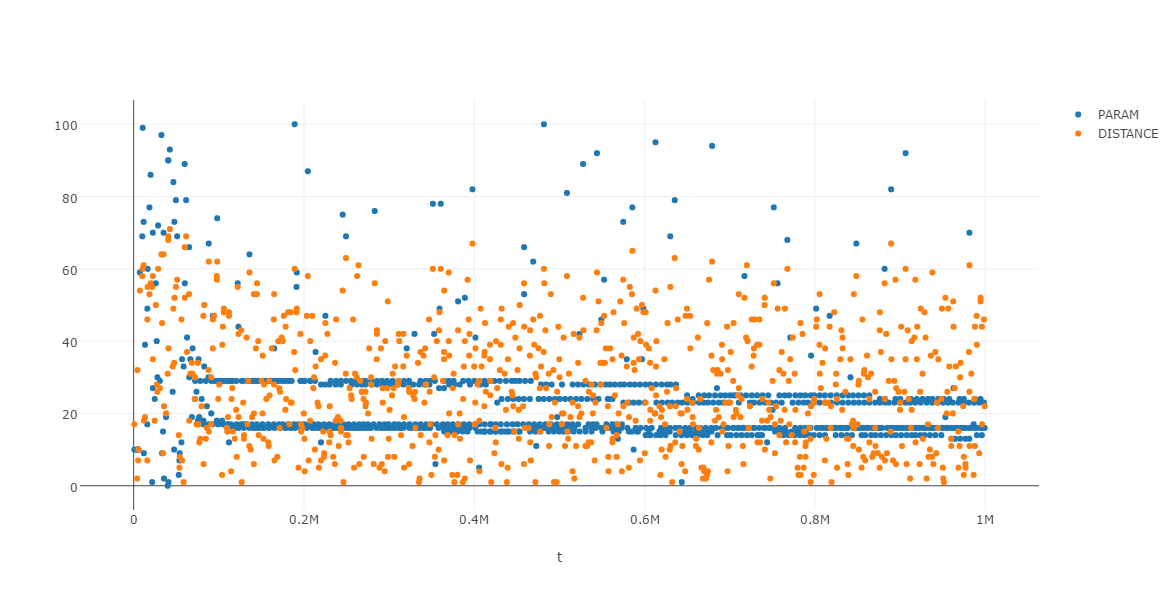
\includegraphics[width=0.8\textwidth]{analyse/SomeMutants/1pm/fixed1some.png}
	\caption{\emph{Fixed-Distance}-Heuristik bei 1 Auto pro Minute und $20\%$ lernenden Fahrern}\label{fig:ap_pm_fd_1}
\end{figure}
\begin{figure}[H]
	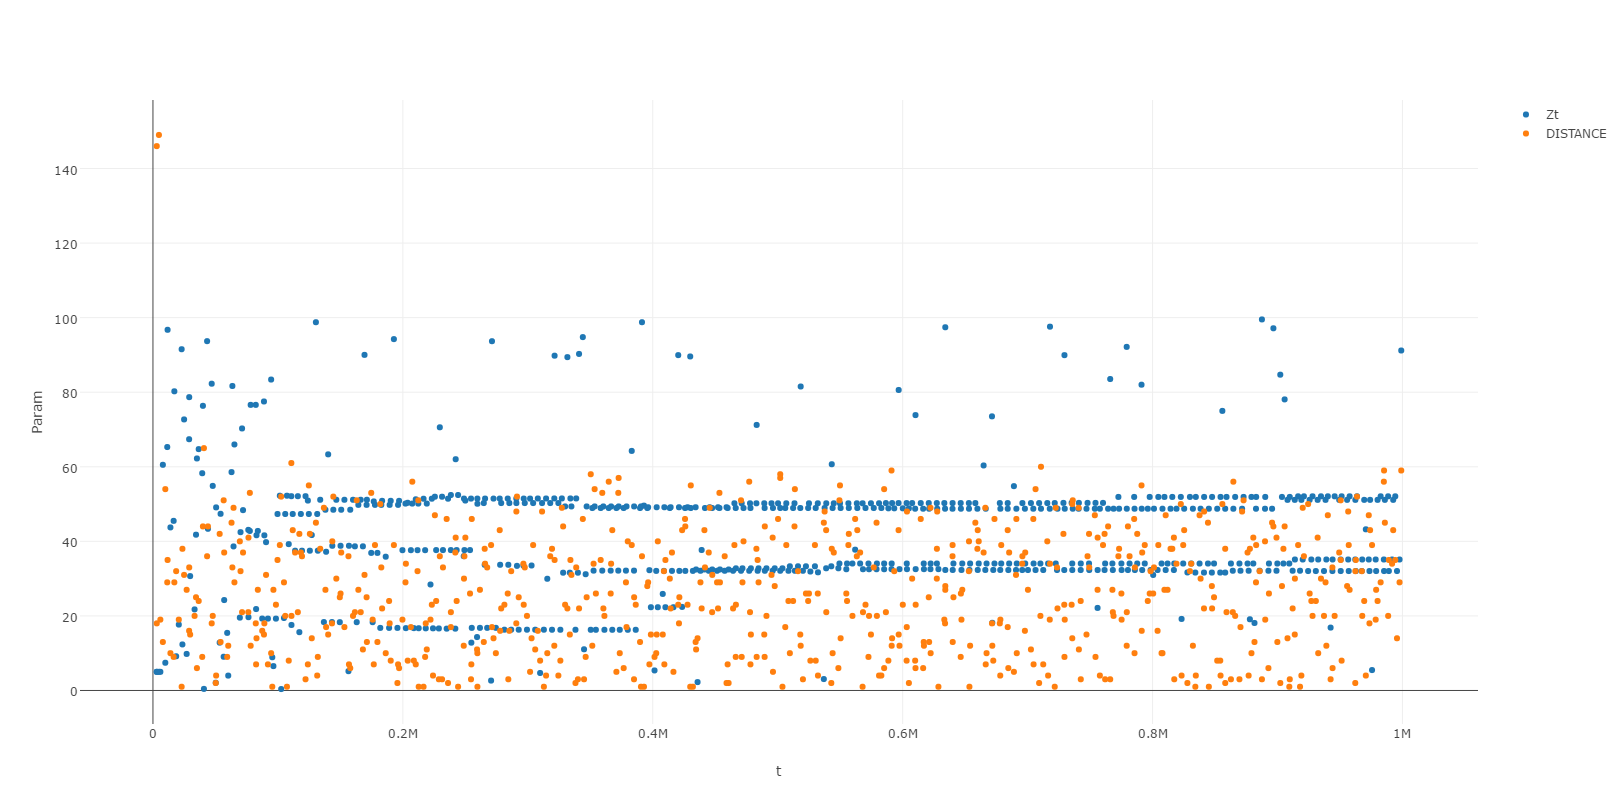
\includegraphics[width=0.8\textwidth]{analyse/SomeMutants/1pm/linop.png}
	\caption{Schranke der \emph{Linear-Operator}-Heuristik bei 1 Auto pro Minute und $20\%$ lernenden Fahrern}\label{fig:ap_pm_loz_1}
\end{figure}
\begin{figure}[H]
	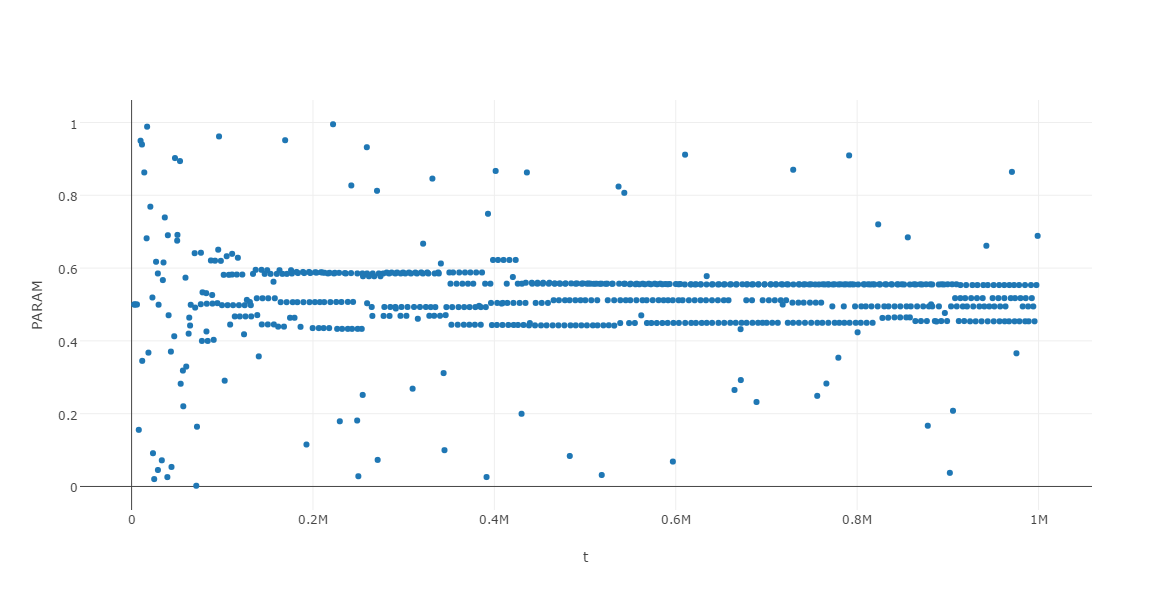
\includegraphics[width=0.8\textwidth]{analyse/SomeMutants/1pm/linopa1some.png}
	\caption{Geschwindigkeit der \emph{Linear-Operator}-Heuristik bei 1 Auto pro Minute und $20\%$ lernenden Fahrern}\label{fig:ap_pm_loa_1}
\end{figure}
\begin{figure}[H]
	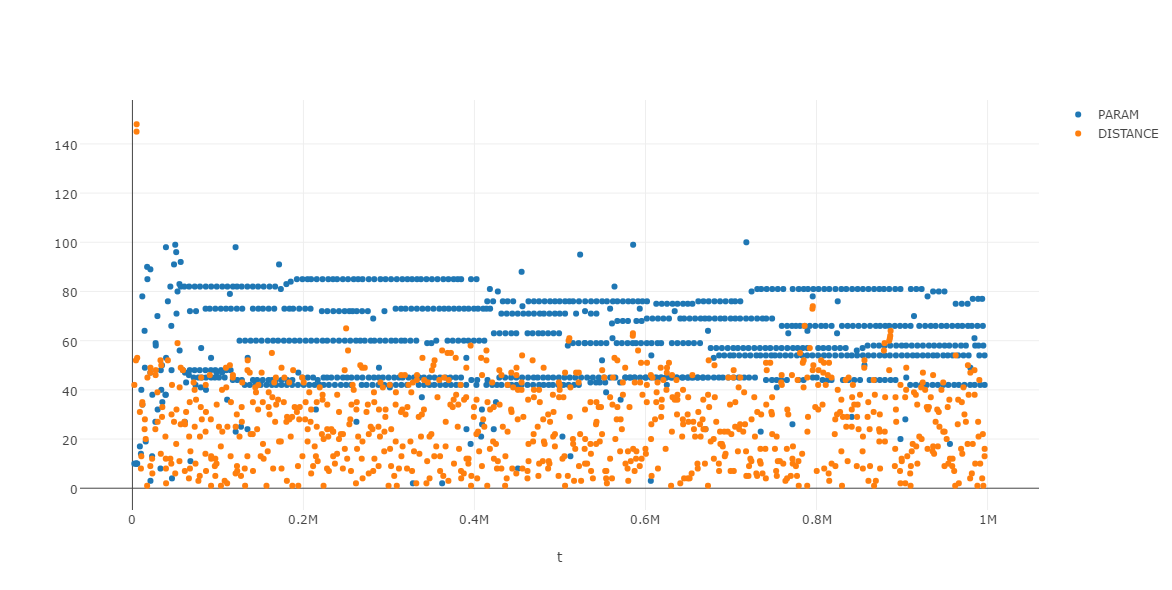
\includegraphics[width=0.8\textwidth]{analyse/SomeMutants/1pm/space1some.png}
	\caption{\emph{Space-Count}-Heuristik bei 1 Auto pro Minute und $20\%$ lernenden Fahrern}\label{fig:ap_pm_sc_1}
\end{figure}
\begin{figure}[H]
	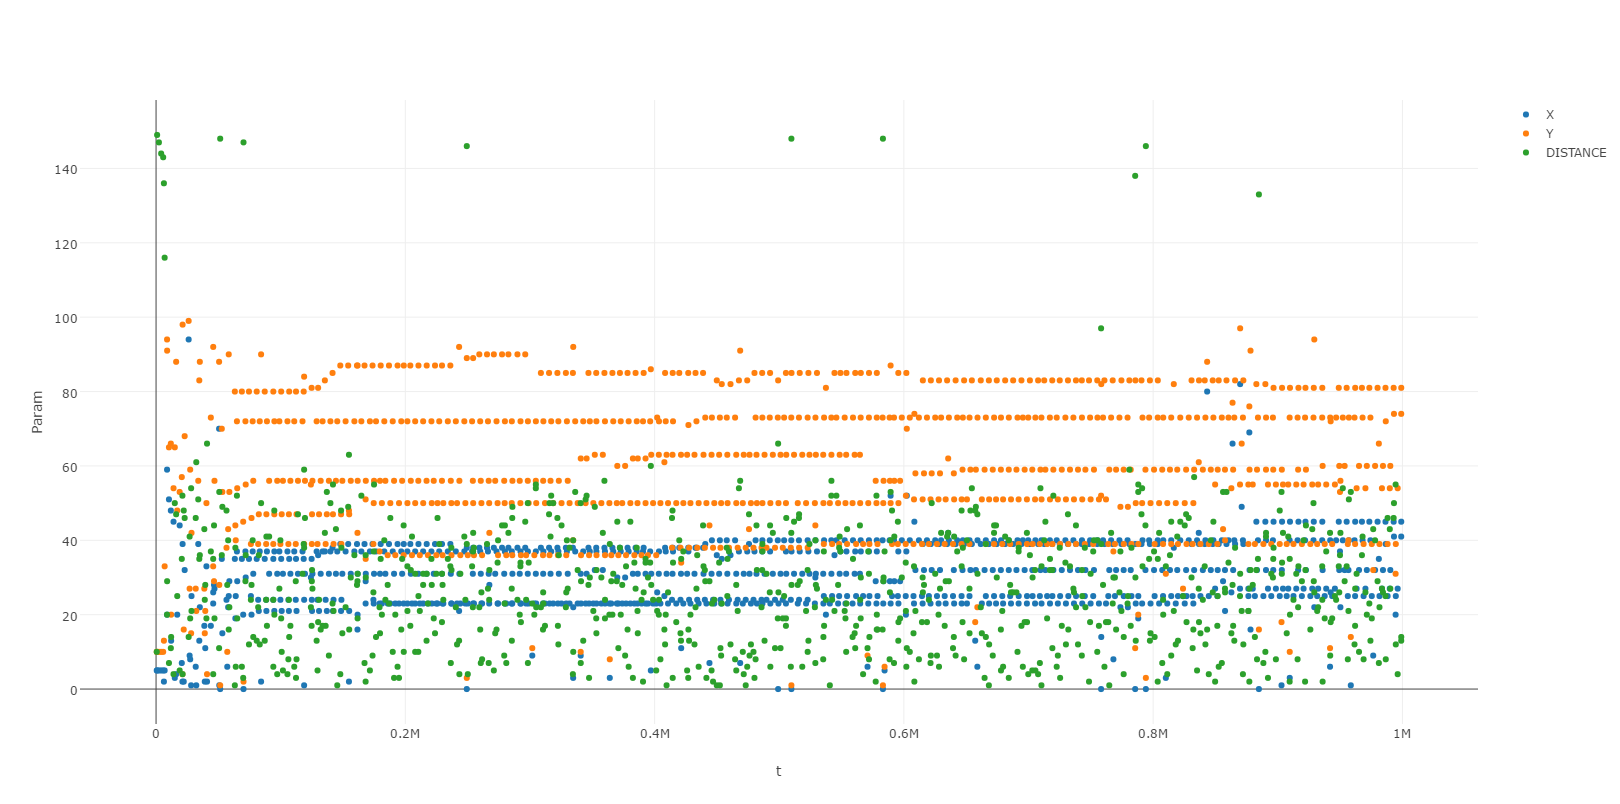
\includegraphics[width=0.8\textwidth]{analyse/SomeMutants/1pm/xy.png}
	\caption{\emph{X-Out-Of-Y}-Heuristik bei 1 Auto pro Minute und $20\%$ lernenden Fahrern}\label{fig:ap_pm_xy_1}
\end{figure}
\begin{figure}[H]
	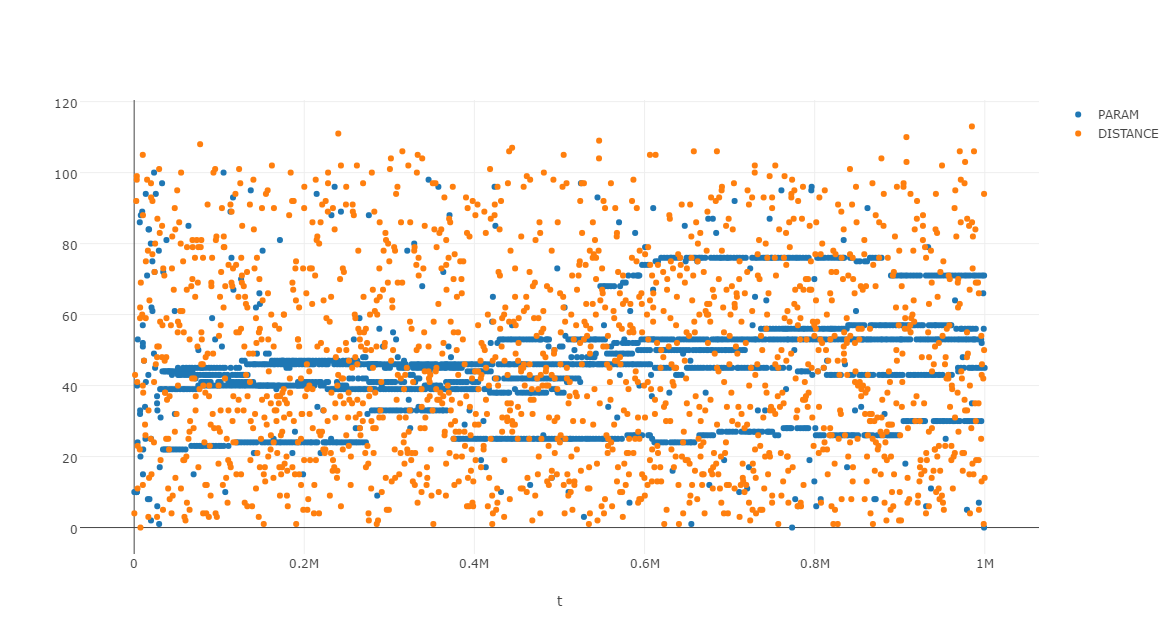
\includegraphics[width=0.8\textwidth]{analyse/SomeMutants/2pm/block2some.png}
	\caption{\emph{Block-Count}-Heuristik bei 2 Autos pro Minute und $20\%$ lernenden Fahrern}\label{fig:ap_pm_bs_2}
\end{figure}
\begin{figure}[H]
	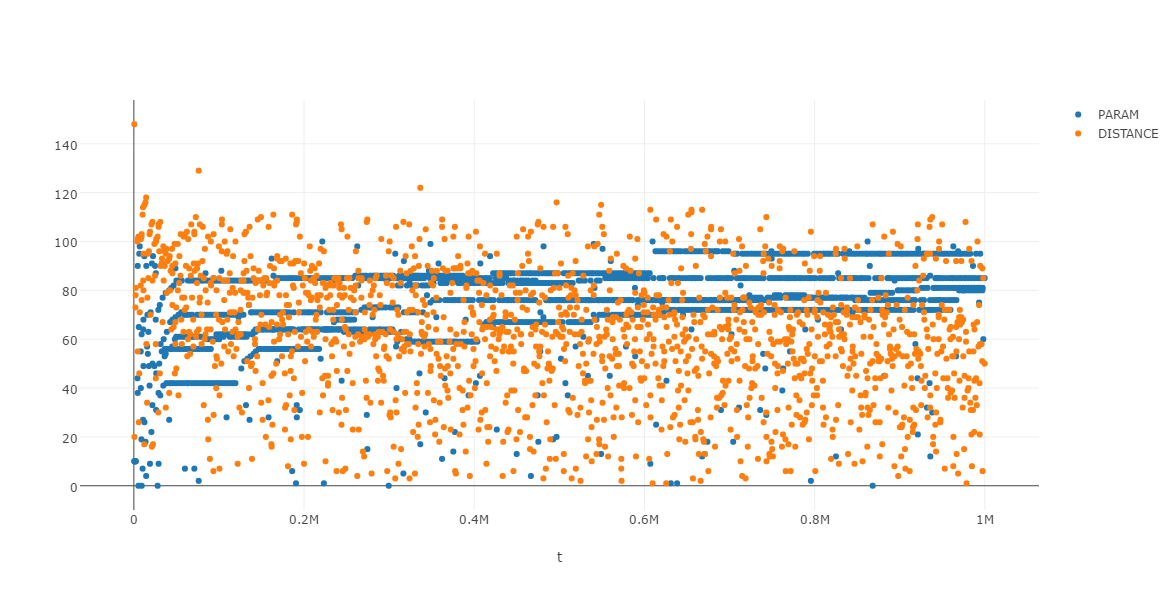
\includegraphics[width=0.8\textwidth]{analyse/SomeMutants/2pm/car2some.png}
	\caption{\emph{Car-Count}-Heuristik bei 2 Autos pro Minute und $20\%$ lernenden Fahrern}\label{fig:ap_pm_cc_2}
\end{figure}
\begin{figure}[H]
	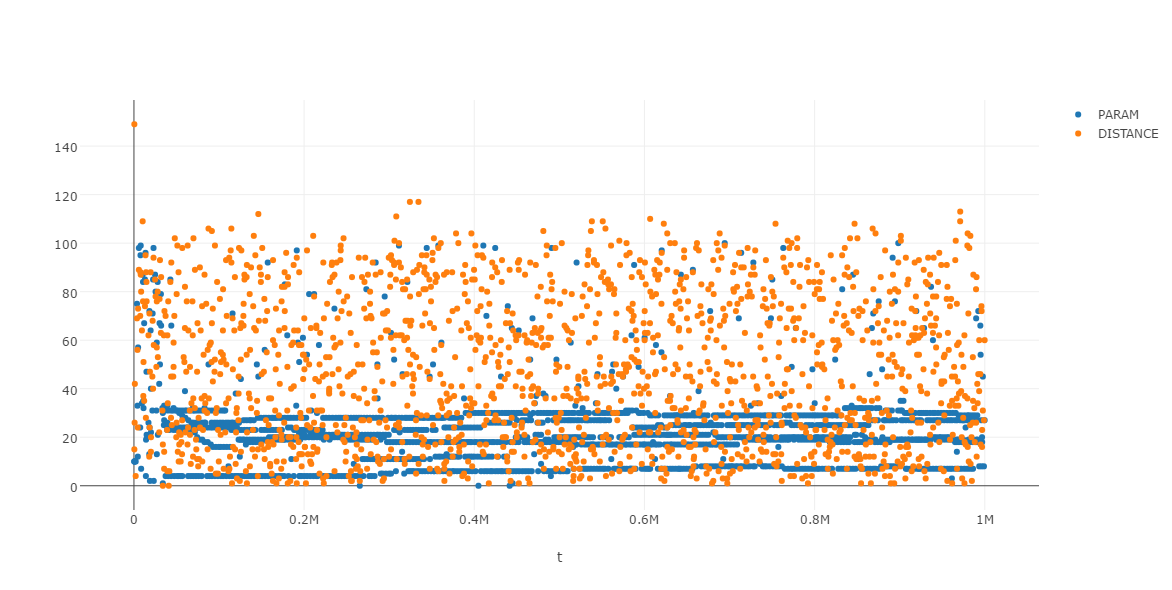
\includegraphics[width=0.8\textwidth]{analyse/SomeMutants/2pm/fixed2some.png}
	\caption{\emph{Fixed-Distance}-Heuristik bei 2 Autos pro Minute und $20\%$ lernenden Fahrern}\label{fig:ap_pm_fd_2}
\end{figure}
\begin{figure}[H]
	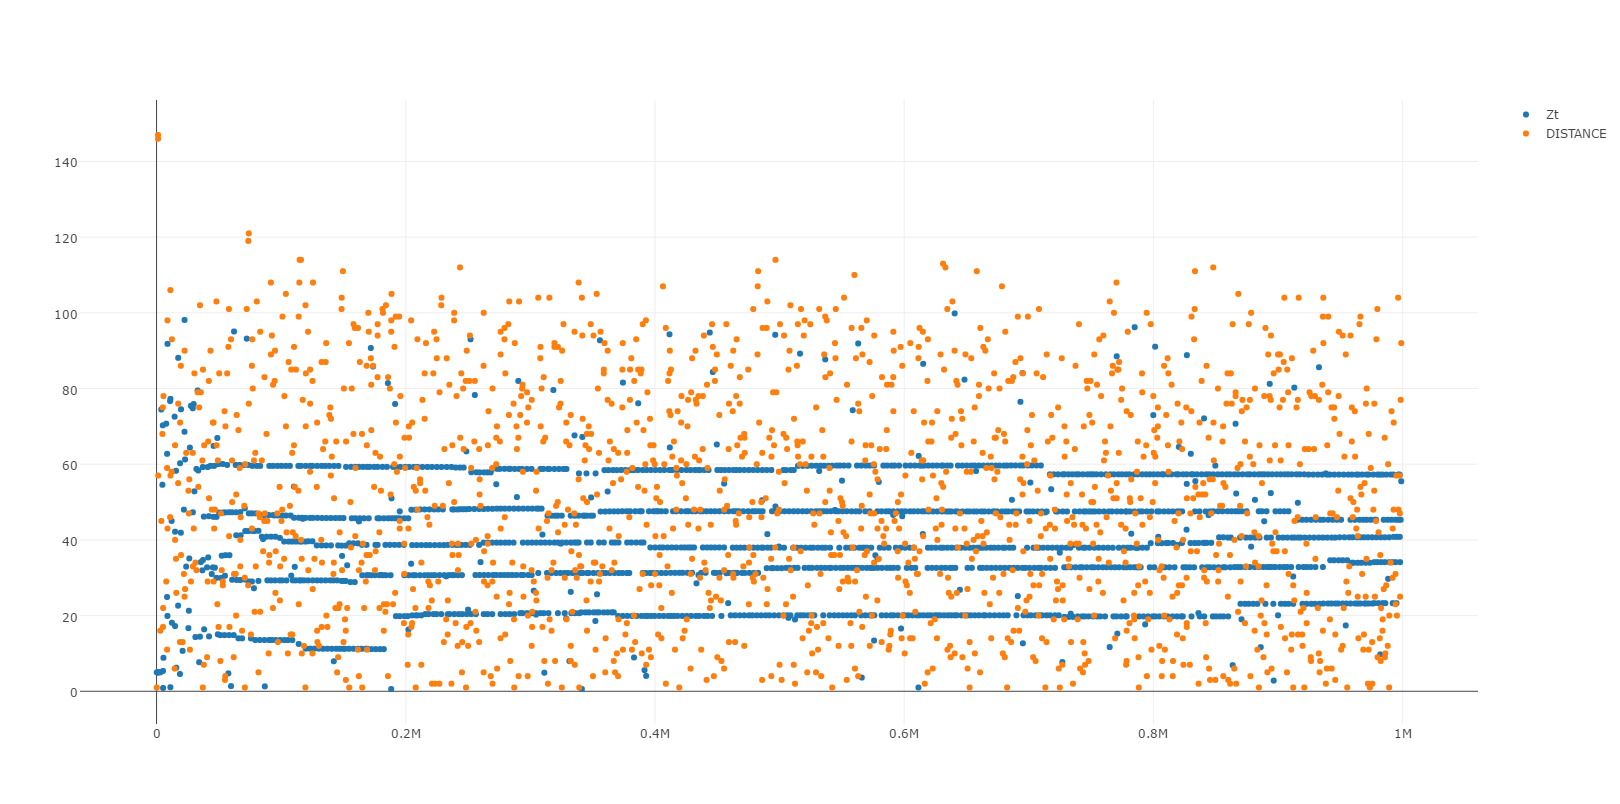
\includegraphics[width=0.8\textwidth]{analyse/SomeMutants/2pm/linop.png}
	\caption{Schranke der \emph{Linear-Operator}-Heuristik bei 2 Autos pro Minute und $20\%$ lernenden Fahrern}\label{fig:ap_pm_loz_2}
\end{figure}
\begin{figure}[H]
	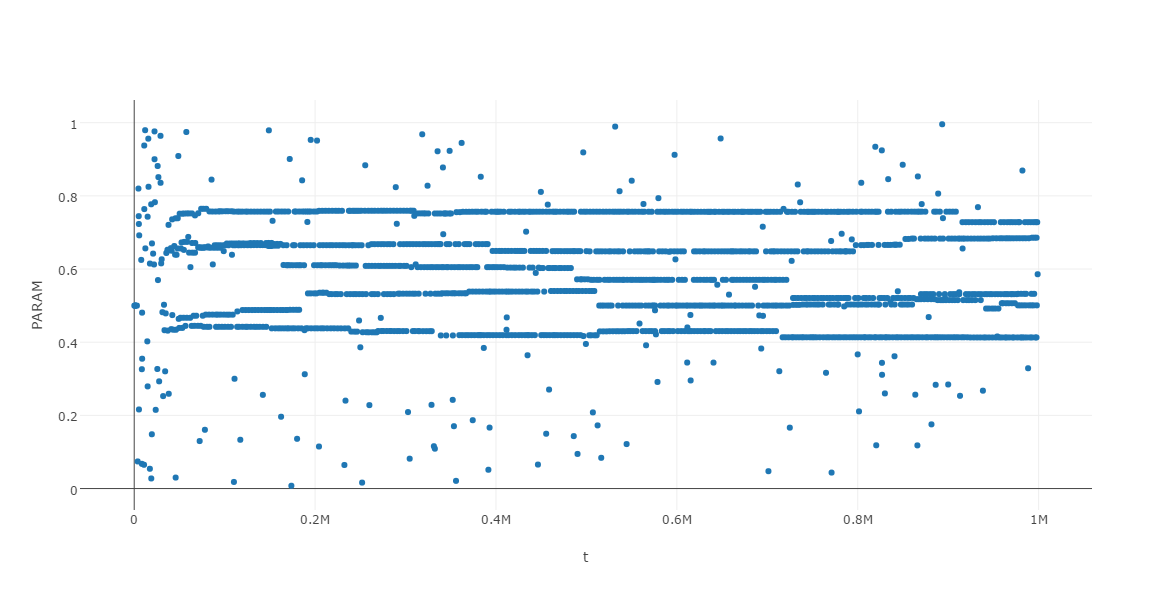
\includegraphics[width=0.8\textwidth]{analyse/SomeMutants/2pm/linopa2some.png}
	\caption{Geschwindigkeit der \emph{Linear-Operator}-Heuristik bei 2 Autos pro Minute und $20\%$ lernenden Fahrern}\label{fig:ap_pm_loa_2}
\end{figure}
\begin{figure}[H]
	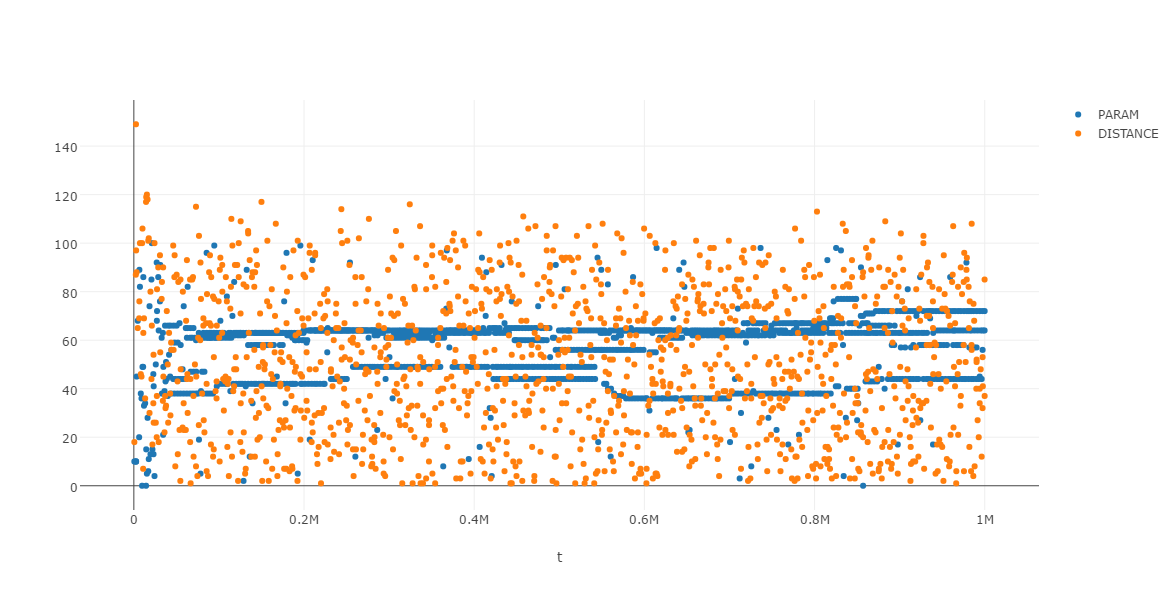
\includegraphics[width=0.8\textwidth]{analyse/SomeMutants/2pm/space2some.png}
	\caption{\emph{Space-Count}-Heuristik bei 2 Autos pro Minute und $20\%$ lernenden Fahrern}\label{fig:ap_pm_sc_2}
\end{figure}
\begin{figure}[H]
	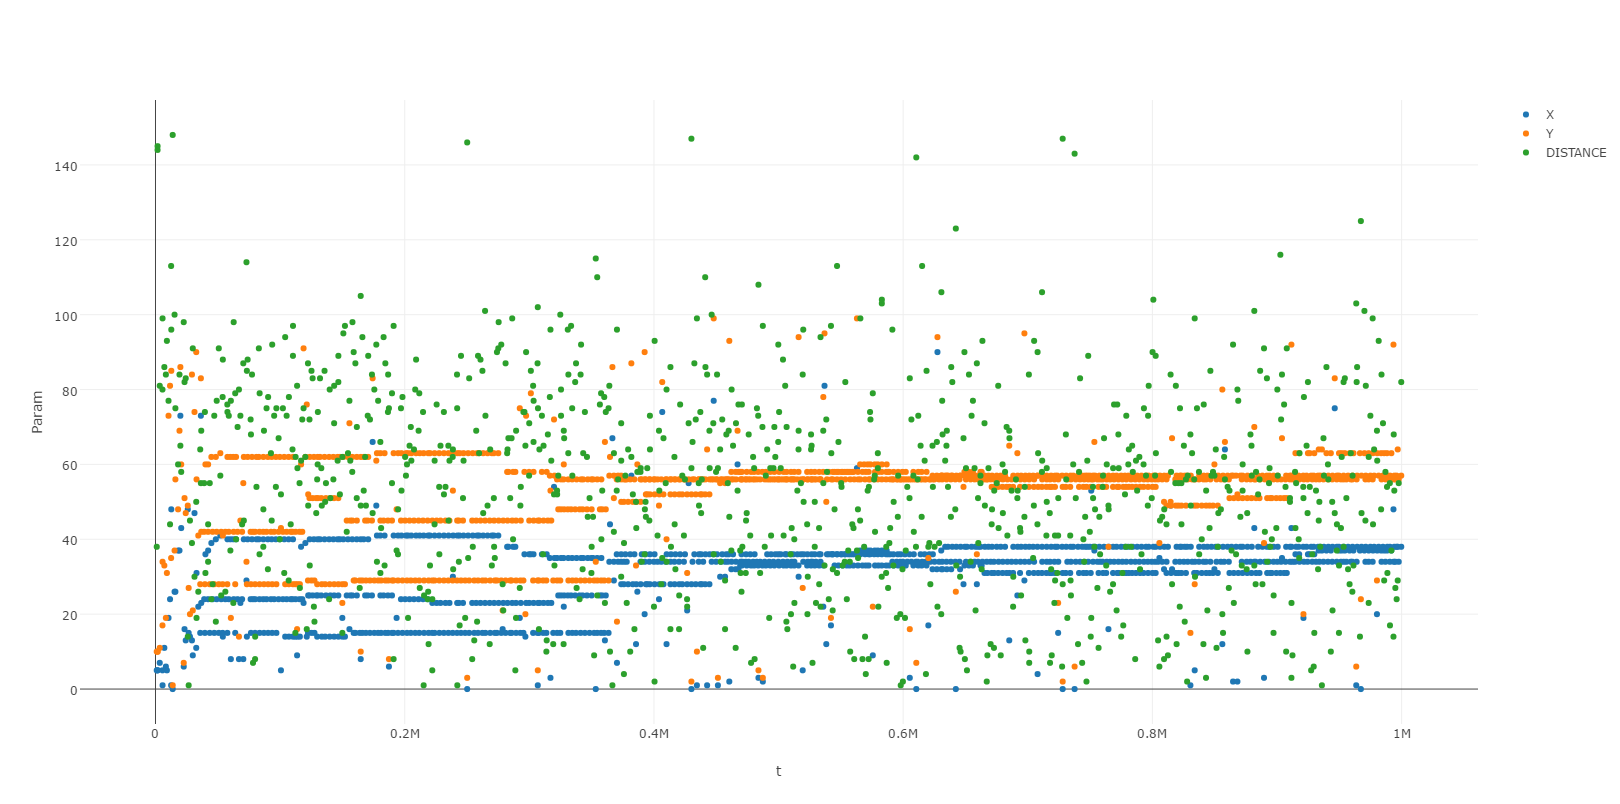
\includegraphics[width=0.8\textwidth]{analyse/SomeMutants/2pm/xy.png}
	\caption{\emph{X-Out-Of-Y}-Heuristik bei 2 Autos pro Minute und $20\%$ lernenden Fahrern}\label{fig:ap_pm_xy_2}
\end{figure}
\begin{figure}[H]
	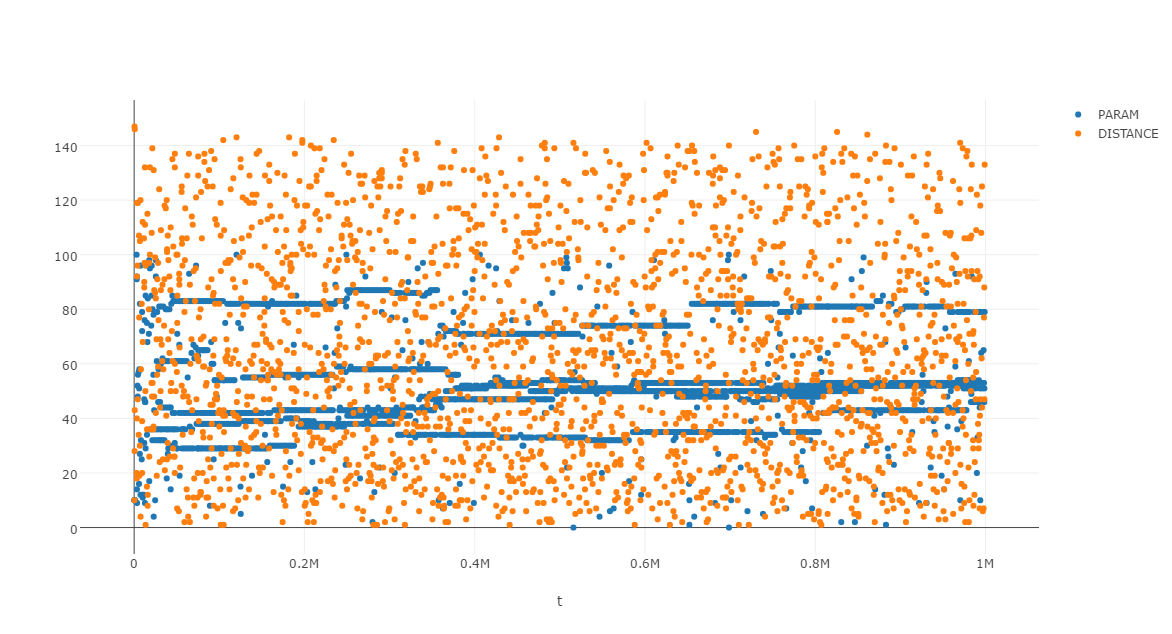
\includegraphics[width=0.8\textwidth]{analyse/SomeMutants/4pm/block4some.png}
	\caption{\emph{Block-Count}-Heuristik bei 4 Autos pro Minute und $20\%$ lernenden Fahrern}\label{fig:ap_pm_bs_4}
\end{figure}
\begin{figure}[H]
	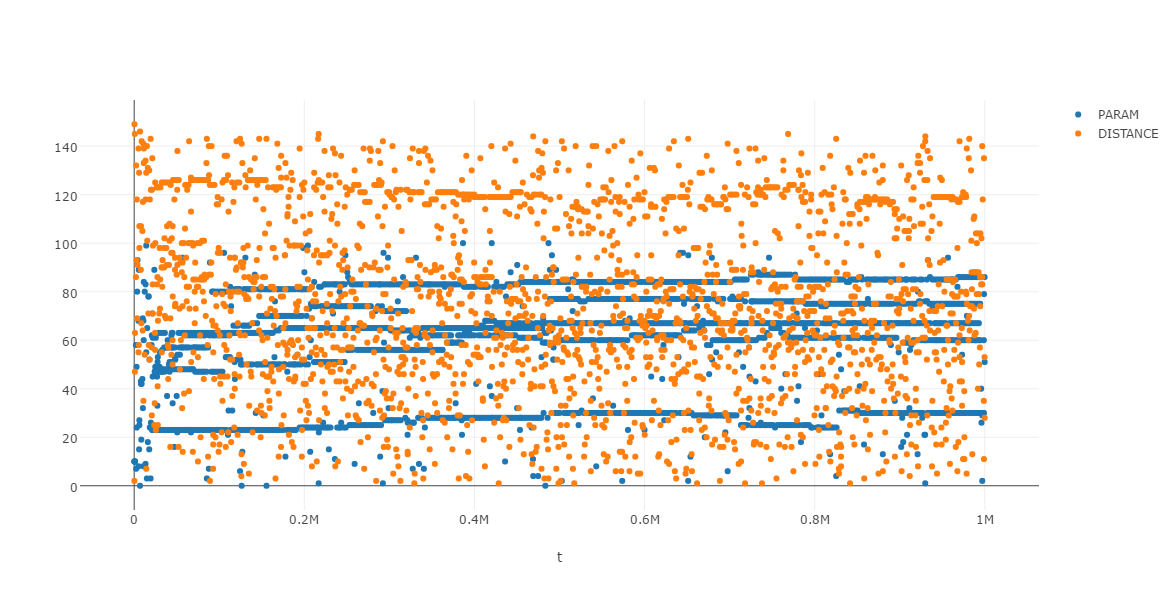
\includegraphics[width=0.8\textwidth]{analyse/SomeMutants/4pm/car4some.png}
	\caption{\emph{Car-Count}-Heuristik bei 4 Autos pro Minute und $20\%$ lernenden Fahrern}\label{fig:ap_pm_cc_4}
\end{figure}
\begin{figure}[H]
	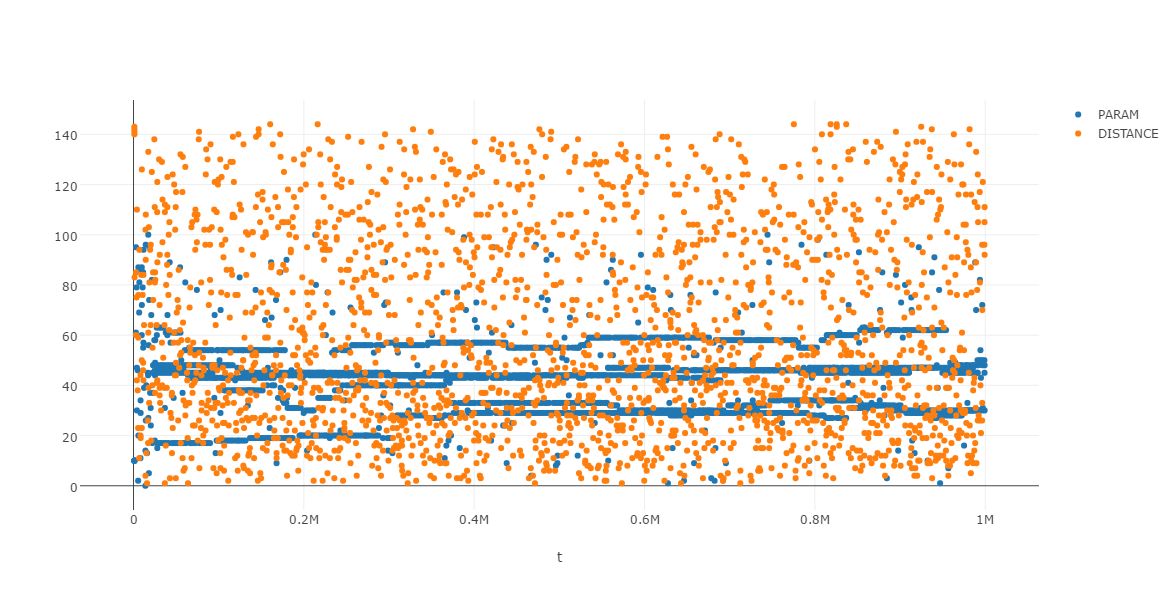
\includegraphics[width=0.8\textwidth]{analyse/SomeMutants/4pm/fixed4some.png}
	\caption{\emph{Fixed-Distance}-Heuristik bei 4 Autos pro Minute und $20\%$ lernenden Fahrern}\label{fig:ap_pm_fd_4}
\end{figure}
\begin{figure}[H]
	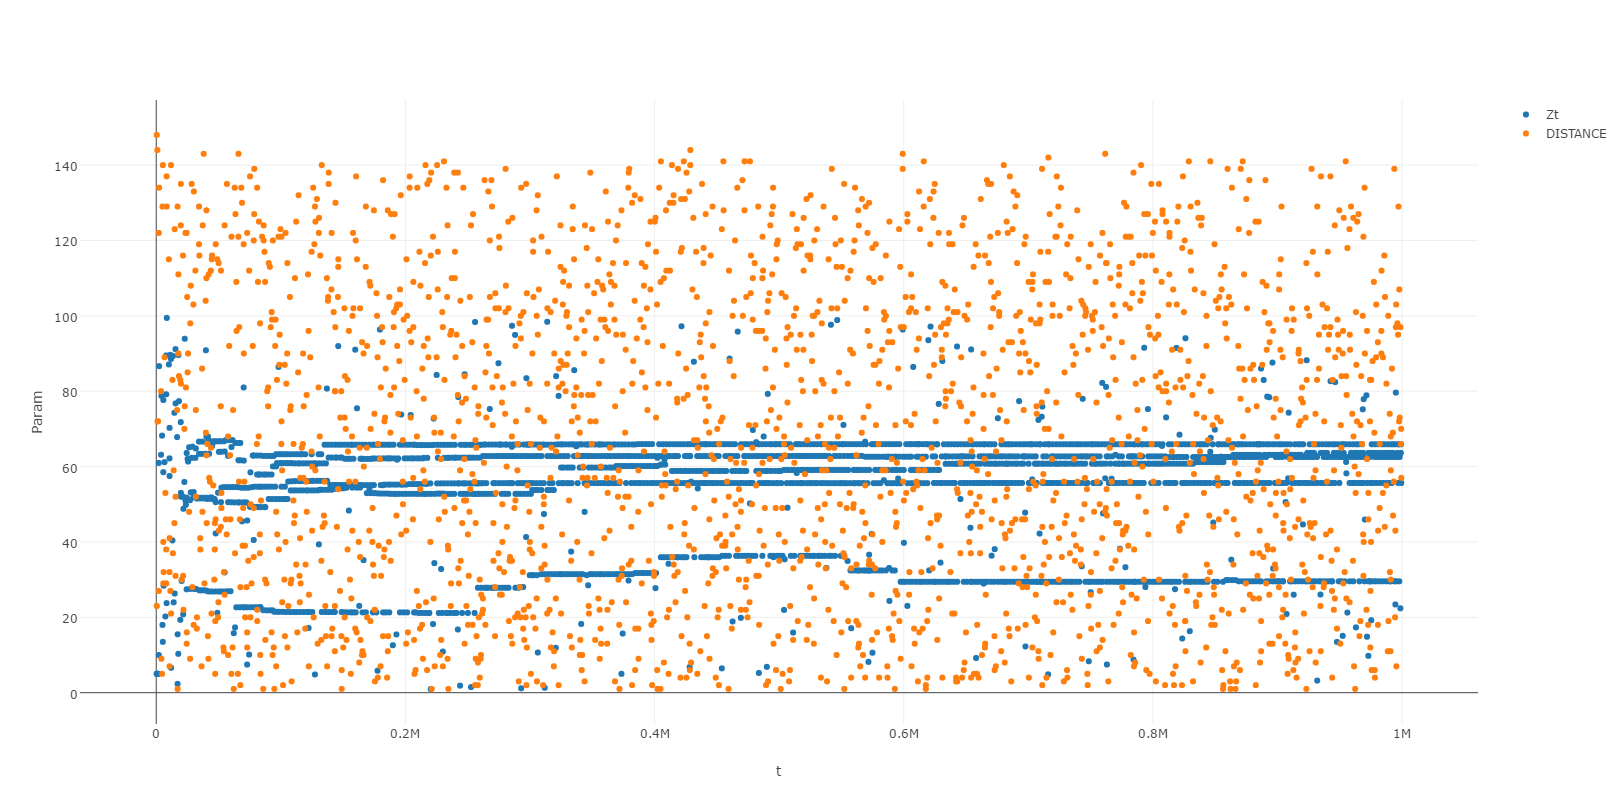
\includegraphics[width=0.8\textwidth]{analyse/SomeMutants/4pm/linop.png}
	\caption{Schranke der \emph{Linear-Operator}-Heuristik bei 4 Autos pro Minute und $20\%$ lernenden Fahrern}\label{fig:ap_pm_loz_4}
\end{figure}
\begin{figure}[H]
	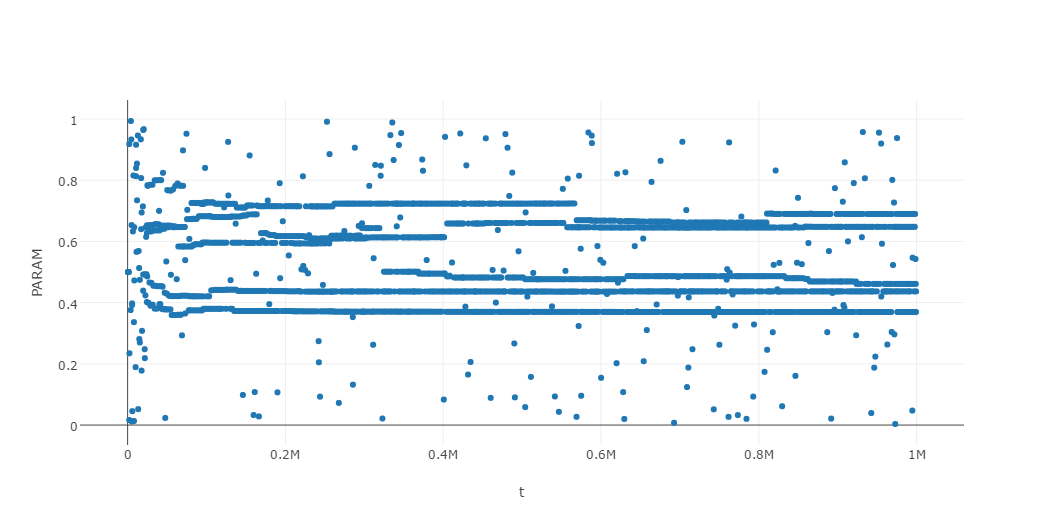
\includegraphics[width=0.8\textwidth]{analyse/SomeMutants/4pm/linopa4some.png}
	\caption{Geschwindigkeit der \emph{Linear-Operator}-Heuristik bei 4 Autos pro Minute und $20\%$ lernenden Fahrern}\label{fig:ap_pm_loa_4}
\end{figure}
\begin{figure}[H]
	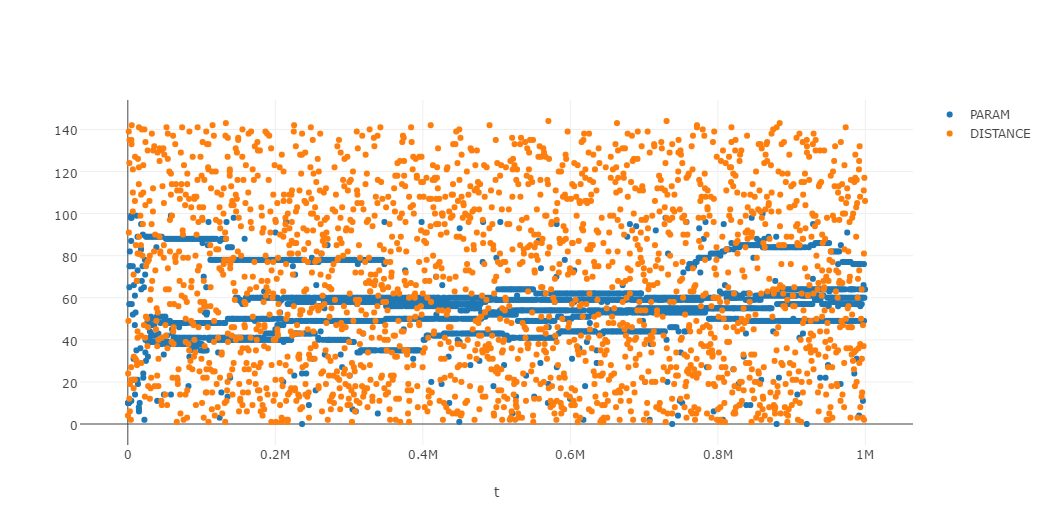
\includegraphics[width=0.8\textwidth]{analyse/SomeMutants/4pm/space4some.png}
	\caption{\emph{Space-Count}-Heuristik bei 4 Autos pro Minute und $20\%$ lernenden Fahrern}\label{fig:ap_pm_sc_4}
\end{figure}
\begin{figure}[H]
	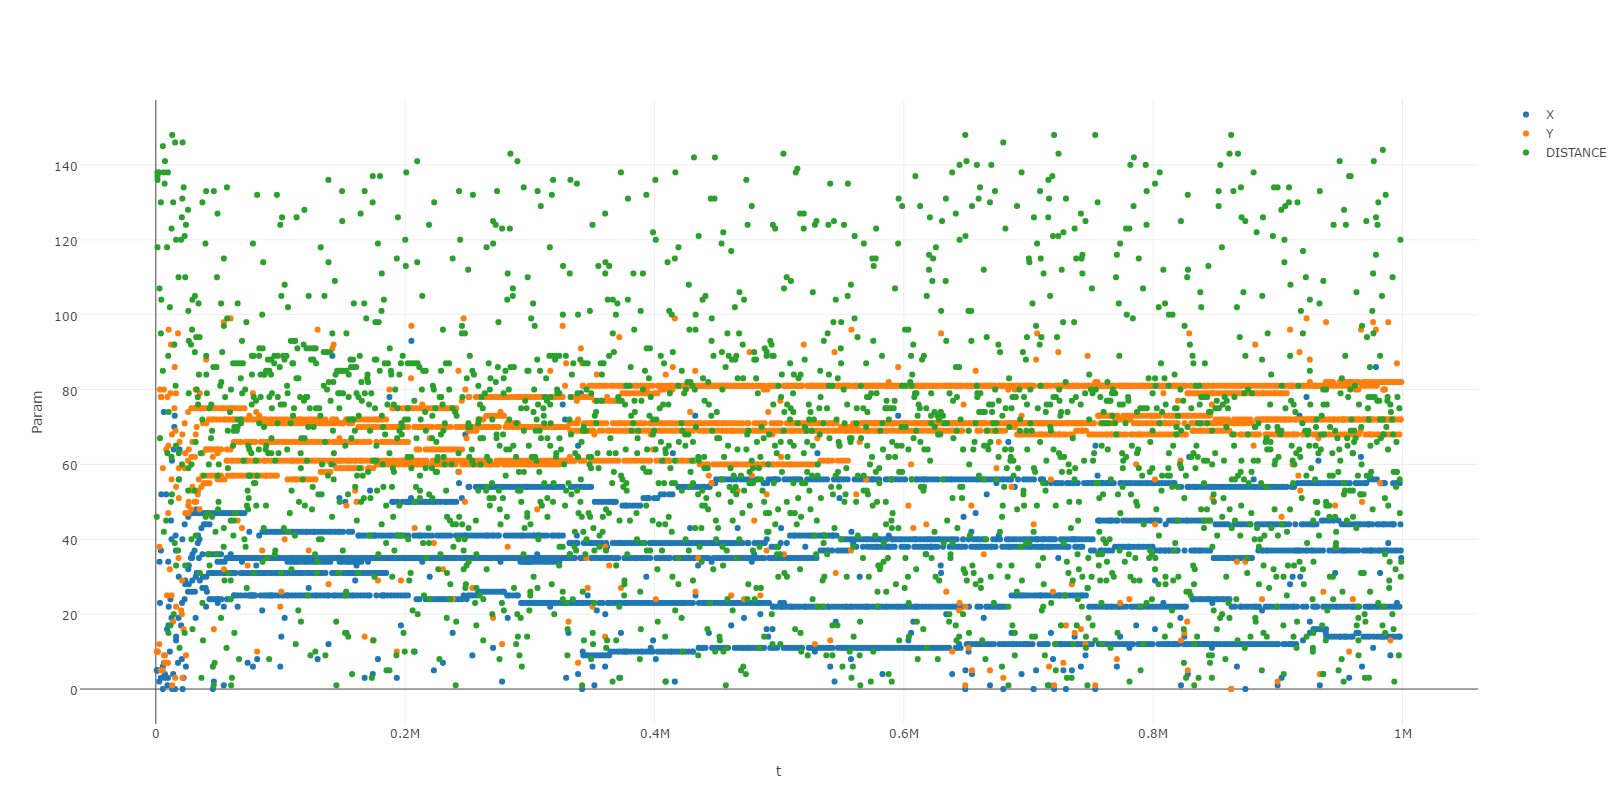
\includegraphics[width=0.8\textwidth]{analyse/SomeMutants/4pm/xy.png}
	\caption{\emph{X-Out-Of-Y}-Heuristik bei 4 Autos pro Minute und $20\%$ lernenden Fahrern}\label{fig:ap_pm_xy_4}
\end{figure}

\subsubsection*{Nur lernende Fahrer}
\begin{figure}[H]
	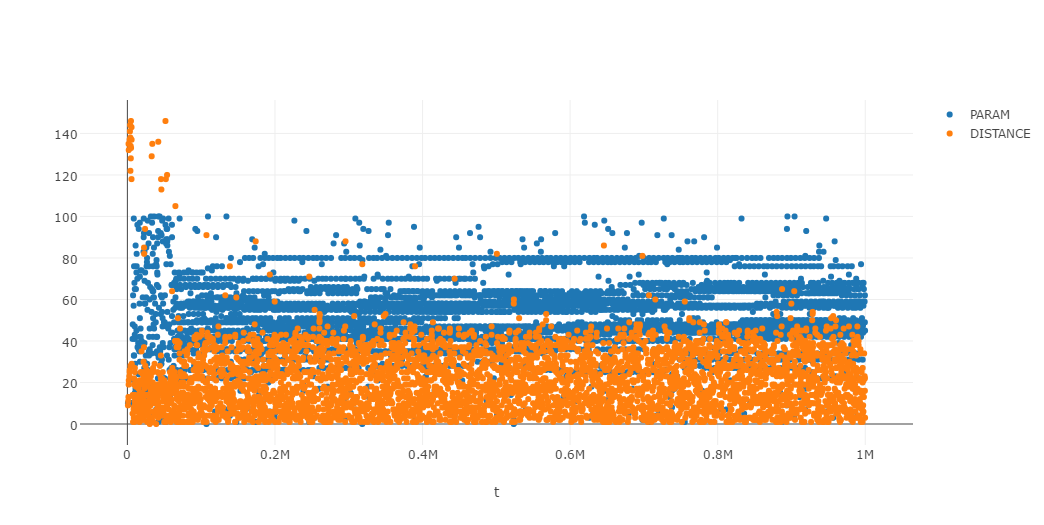
\includegraphics[width=0.8\textwidth]{analyse/JustHeuristik/1pm/block1just.png}
	\caption{\emph{Block-Count}-Heuristik bei 1 Auto pro Minute und nur lernende Fahrer}\label{fig:ap_jh_bs_1}
\end{figure}
\begin{figure}[H]
	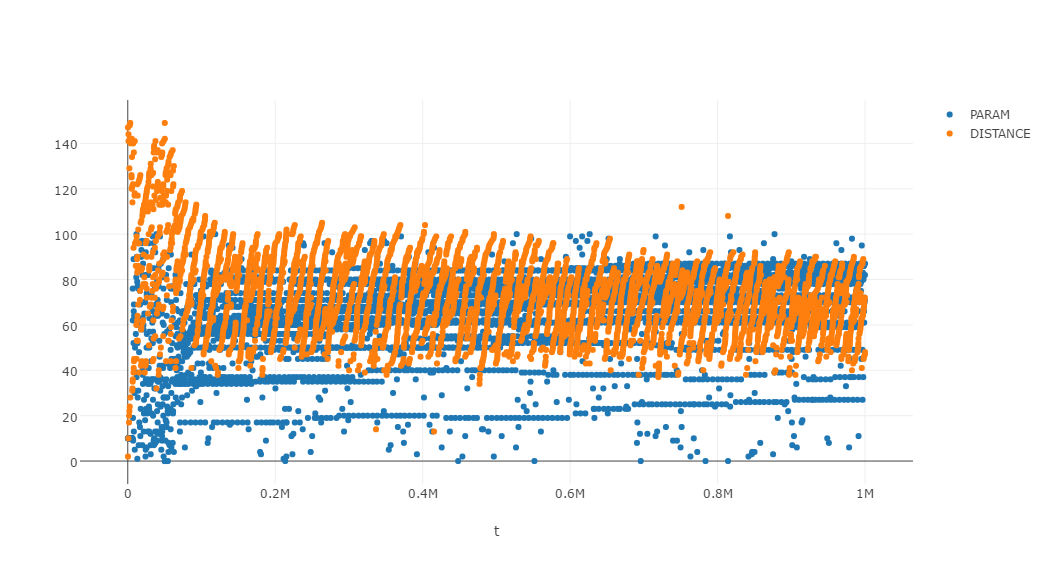
\includegraphics[width=0.8\textwidth]{analyse/JustHeuristik/1pm/car1just.png}
	\caption{\emph{Car-Count}-Heuristik bei 1 Auto pro Minute und nur lernende Fahrer}\label{fig:ap_jh_cc_1}
\end{figure}
\begin{figure}[H]
	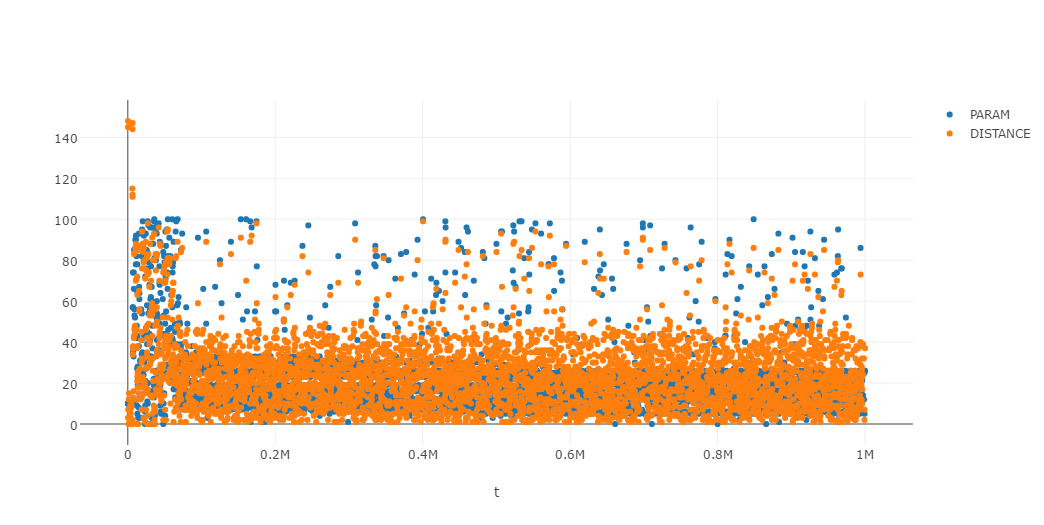
\includegraphics[width=0.8\textwidth]{analyse/JustHeuristik/1pm/fixed1just.png}
	\caption{\emph{Fixed-Distance}-Heuristik bei 1 Auto pro Minute und nur lernende Fahrer}\label{fig:ap_jh_fd_1}
\end{figure}
\begin{figure}[H]
	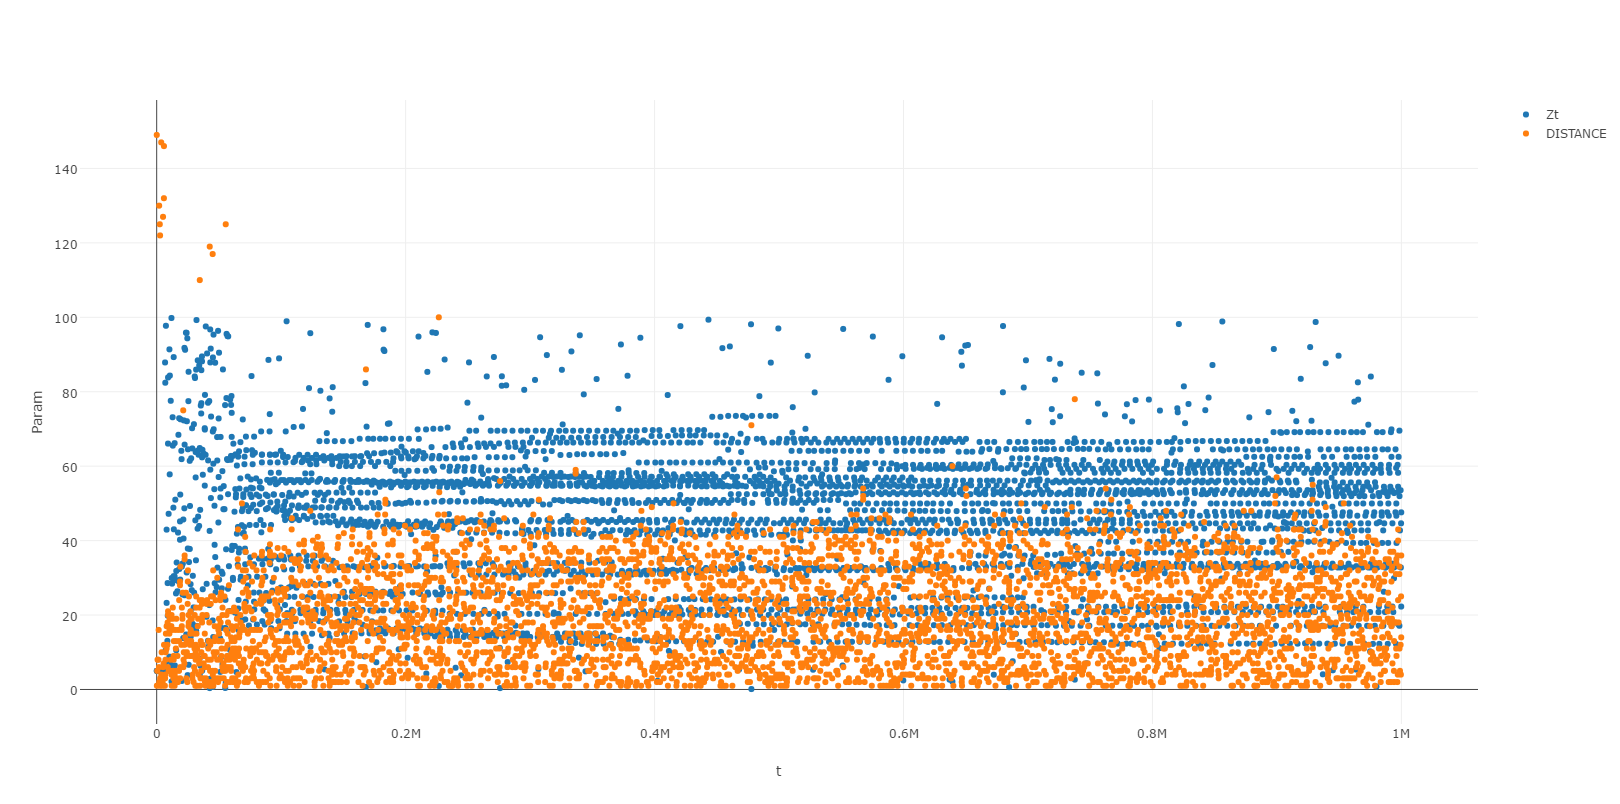
\includegraphics[width=0.8\textwidth]{analyse/JustHeuristik/1pm/linop.png}
	\caption{Schranke der \emph{Linear-Operator}-Heuristik bei 1 Auto pro Minute und nur lernende Fahrer}\label{fig:ap_jh_loz_1}
\end{figure}
\begin{figure}[H]
	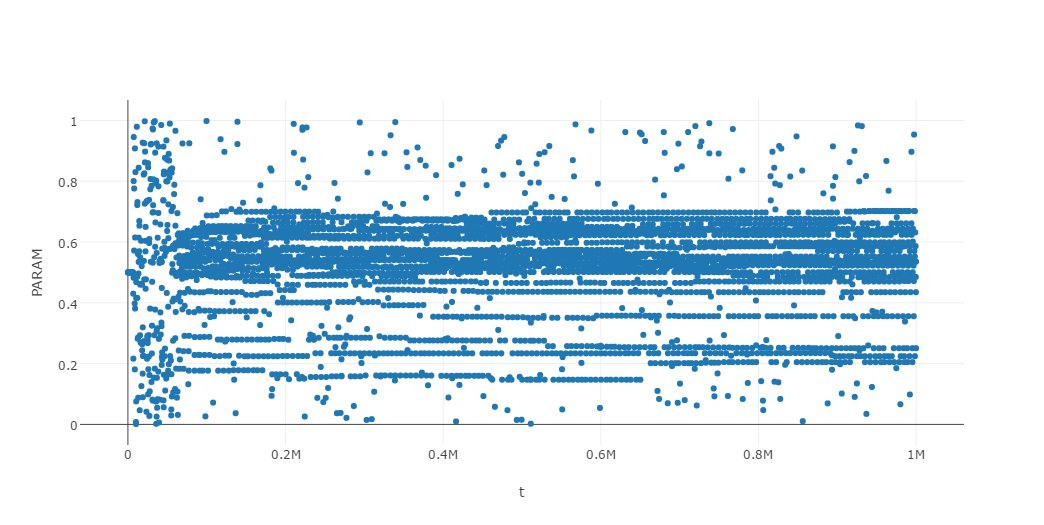
\includegraphics[width=0.8\textwidth]{analyse/JustHeuristik/1pm/linopa1just.png}
	\caption{Geschwindigkeit der \emph{Linear-Operator}-Heuristik bei 1 Auto pro Minute und nur lernende Fahrer}\label{fig:ap_jh_loa_1}
\end{figure}
\begin{figure}[H]
	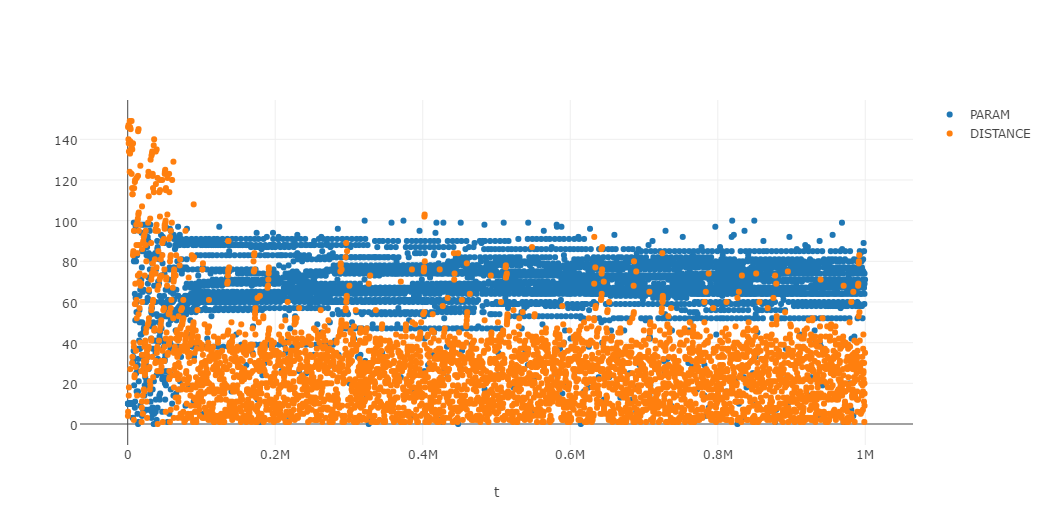
\includegraphics[width=0.8\textwidth]{analyse/JustHeuristik/1pm/space1just.png}
	\caption{\emph{Space-Count}-Heuristik bei 1 Auto pro Minute und nur lernende Fahrer}\label{fig:ap_jh_sc_1}
\end{figure}
\begin{figure}[H]
	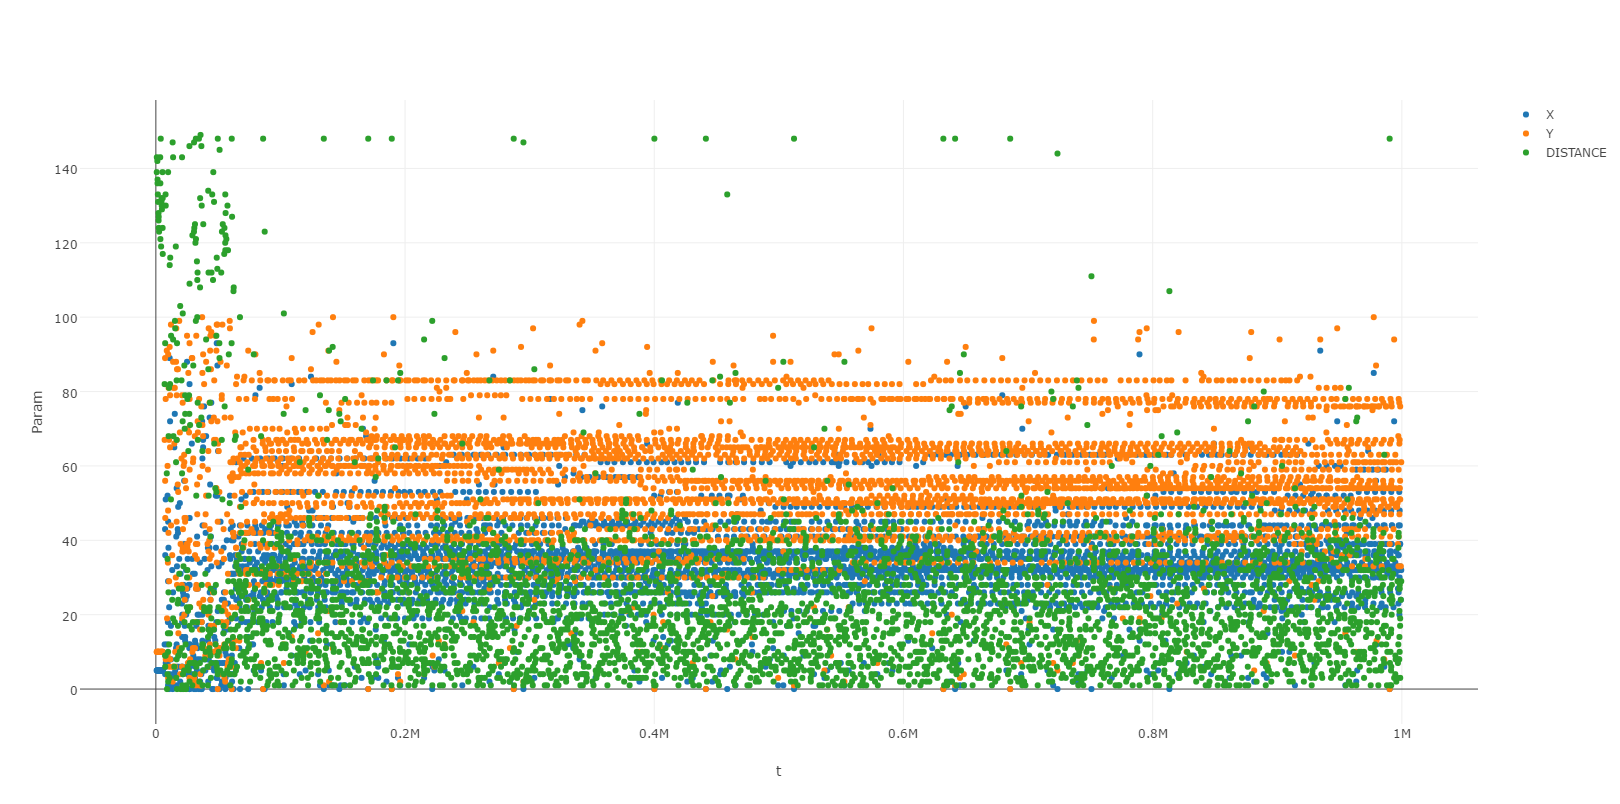
\includegraphics[width=0.8\textwidth]{analyse/JustHeuristik/1pm/xy.png}
	\caption{\emph{X-Out-Of-Y}-Heuristik bei 1 Auto pro Minute und nur lernende Fahrer}\label{fig:ap_jh_xy_1}
\end{figure}
\begin{figure}[H]
	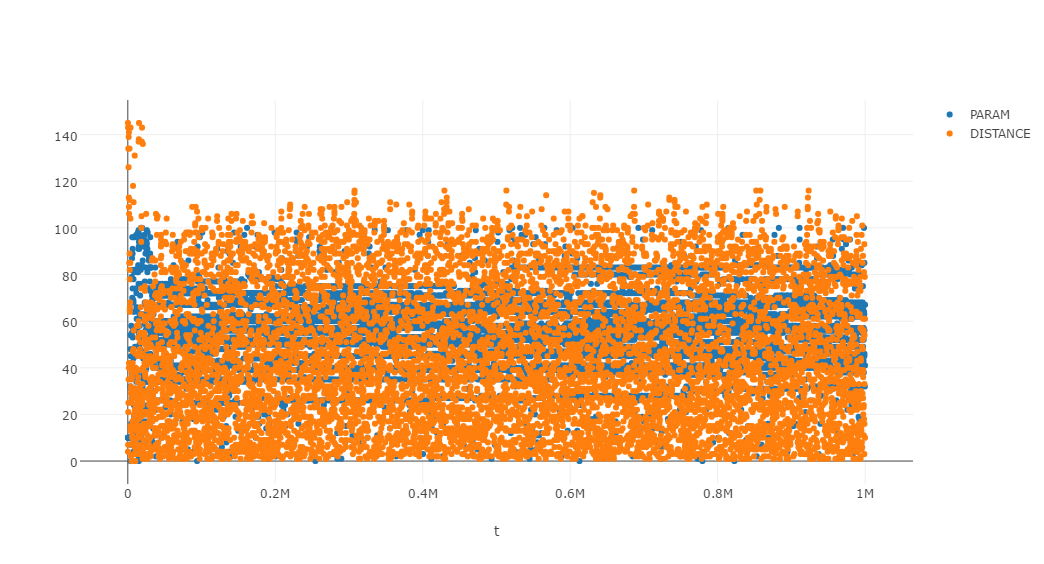
\includegraphics[width=0.8\textwidth]{analyse/JustHeuristik/2pm/block2just.png}
	\caption{\emph{Block-Count}-Heuristik bei 2 Autos pro Minute und nur lernende Fahrer}\label{fig:ap_jh_bs_2}
\end{figure}
\begin{figure}[H]
	\includegraphics[width=0.8\textwidth]{analyse/JustHeuristik/2pm/car2just.png}
	\caption{\emph{Car-Count}-Heuristik bei 2 Autos pro Minute und nur lernende Fahrer}\label{fig:ap_jh_cc_2}
\end{figure}
\begin{figure}[H]
	\includegraphics[width=0.8\textwidth]{analyse/JustHeuristik/2pm/fixed2just.png}
	\caption{\emph{Fixed-Distance}-Heuristik bei 2 Autos pro Minute und nur lernende Fahrer}\label{fig:ap_jh_fd_2}
\end{figure}
\begin{figure}[H]
	\includegraphics[width=0.8\textwidth]{analyse/JustHeuristik/2pm/linop.png}
	\caption{Schranke der \emph{Linear-Operator}-Heuristik bei 2 Autos pro Minute und nur lernende Fahrer}\label{fig:ap_jh_loz_2}
\end{figure}
\begin{figure}[H]
	\includegraphics[width=0.8\textwidth]{analyse/JustHeuristik/2pm/linopa2just.png}
	\caption{Geschwindigkeit der \emph{Linear-Operator}-Heuristik bei 2 Autos pro Minute und nur lernende Fahrer}\label{fig:ap_jh_loa_2}
\end{figure}
\begin{figure}[H]
	\includegraphics[width=0.8\textwidth]{analyse/JustHeuristik/2pm/space2just.png}
	\caption{\emph{Space-Count}-Heuristik bei 2 Autos pro Minute und nur lernende Fahrer}\label{fig:ap_jh_sc_2}
\end{figure}
\begin{figure}[H]
	\includegraphics[width=0.8\textwidth]{analyse/JustHeuristik/2pm/xy.png}
	\caption{\emph{X-Out-Of-Y}-Heuristik bei 2 Autos pro Minute und nur lernende Fahrer}\label{fig:ap_jh_xy_2}
\end{figure}
\begin{figure}[H]
	\includegraphics[width=0.8\textwidth]{analyse/JustHeuristik/4pm/block4just.png}
	\caption{\emph{Block-Count}-Heuristik bei 4 Autos pro Minute und nur lernende Fahrer}\label{fig:ap_jh_bs_4}
\end{figure}
\begin{figure}[H]
	\includegraphics[width=0.8\textwidth]{analyse/JustHeuristik/4pm/car4just.png}
	\caption{\emph{Car-Count}-Heuristik bei 4 Autos pro Minute und nur lernende Fahrer}\label{fig:ap_jh_cc_4}
\end{figure}
\begin{figure}[H]
	\includegraphics[width=0.8\textwidth]{analyse/JustHeuristik/4pm/fixed4just.png}
	\caption{\emph{Fixed-Distance}-Heuristik bei 4 Autos pro Minute und nur lernende Fahrer}\label{fig:ap_jh_fd_4}
\end{figure}
\begin{figure}[H]
	\includegraphics[width=0.8\textwidth]{analyse/JustHeuristik/4pm/linop.png}
	\caption{Schranke der \emph{Linear-Operator}-Heuristik bei 4 Autos pro Minute und nur lernende Fahrer}\label{fig:ap_jh_loz_4}
\end{figure}
\begin{figure}[H]
	\includegraphics[width=0.8\textwidth]{analyse/JustHeuristik/4pm/linopa4just.png}
	\caption{Geschwindigkeit der \emph{Linear-Operator}-Heuristik bei 4 Autos pro Minute und nur lernende Fahrer}\label{fig:ap_jh_loa_4}
\end{figure}
\begin{figure}[H]
	\includegraphics[width=0.8\textwidth]{analyse/JustHeuristik/4pm/space4just.png}
	\caption{\emph{Space-Count}-Heuristik bei 4 Autos pro Minute und nur lernende Fahrer}\label{fig:ap_jh_sc_4}
\end{figure}
\begin{figure}[H]
	\includegraphics[width=0.8\textwidth]{analyse/JustHeuristik/4pm/xy.png}
	\caption{\emph{X-Out-Of-Y}-Heuristik bei 4 Autos pro Minute und nur lernende Fahrer}\label{fig:ap_jh_xy_4}
\end{figure}